\chapter{Sviluppo della soluzione Equiticket come risposta al Secondary Ticketing}
Il capitolo \ref{chap:equiticket} ha lo scopo di mostrare il contributo apportato dal candidato alla soluzione proposta. La struttura della presentazione segue quella già enunciata nella Sezione \ref{sec:sommario}.
\label{chap:equiticket}
\section{Background economico e origine della soluzione} \label{sec:background}
Il capitolo ha lo scopo di presentare il vero e proprio contributo personale dell'autore della tesi: la contribuzione allo sviluppo della piattaforma \emph{\textbf{Equiticket}}, prima start-up in Italia a presentarsi come alternativa concreta al Secondary Ticketing. \\*
\`E oppurtuno sottolineare il fatto che il progetto si concentri principalmente sul combattere la rivendita di titoli di accesso a prezzo maggiorato, che, come è stato dimostrato nei capitoli \ref{chap:stato_arte} e \ref{chap:best_p}, danneggia pesantemente il mercato, gli artisti e i consumatori, oltre che a creare problemi al territorio e al fisco. \\
Equiticket (logo in Figura \ref{logoequi}) si presenta come un portale dove ogni utente può rivendere il suo biglietto con la condizione che la cifra richiesta sia minore o uguale al prezzo di emissione, in modo da disincentivare la speculazione tra utenti. 
%Inserire logo Equiticket e immagine della pagina
\begin{figure}[htbp]
	\centering
	
\includegraphics[width=0.68\textwidth]{chapter4/immagini/logo300}
	\caption{Logo di Equiticket}
	\label{logoequi}
\end{figure}
Sebbene Equiticket nasca come portale di \textit{rivendita}, dedicato alla cessione e all'acquisto di biglietti già precedentemente acquistati, a partire dal 15 Aprile 2019 esso è diventato anche un portale primario autorizzato per la vendita di titoli di accesso. 
Tale estensione di linea è stata possibile grazie all'integrazione nel Sistema Informatico di una suite software, approvata da \textit{SIAE} e \textit{Agenzia delle Entrate}, detta \emph{Misuratore Fiscale}. \\
Tale software permette l'integrazione col sistema fiscale italiano e permette di gestire le vendite sul mercato primario secondo diverse formule: oltre le vendite dei titoli di accesso, i misuratori permettono anche la vendita di diverse tipologie di eventi, oltre che abbinamenti con altre tipologie di prodotti (es. merchandising, pacchetti comprensivi di alberghi, incontri esclusivi ecc.).
Al momento della progettazione del sistema di vendita primario, è possibile scegliere se implementare un Misuratore fiscale proprietario, sviluppato ad-hoc per la piattaforma, oppure integrarne uno già esistente tra quelli disponibili sul mercato. 
La decisione presa da Equiticket è stata quella di integrare, per la fase iniziale del progetto, il Misuratore sviluppato da \textit{MTicket} (parte di \textit{MMM Group}), società italiana con sede a Milano: parallelamente, è iniziato anche lo sviluppo di un Misuratore Fiscale proprietario, la cui realizzazione è prevista tra la fine del 2019 e i primi mesi del 2020. 
\\
Equiticket si avvale di un'architettura software sviluppata completamente in ambiente Cloud, oltre che di una logica anti-truffa proprietaria e sviluppata in modo tale da garantire al consumatore finale la migliore esperienza di acquisto possibile. 
Equiticket è stato rilasciato nell'Aprile del 2018 e, pochi mesi dopo, a cavallo tra Ottobre 2018 e Febbraio 2019, ha ricevuto finanziamenti esterni per una quota di circa 233.000€ tramite una campagna di \textit{\emph{Equity Crowdfunding}} sul portale \textit{\emph{Opstart}}, portale specializzato nella ricerca di finanziamenti per start-up e PMI.
Una volta appurata l'impossibilità, come discusso nel capitolo precedente, di fronteggiare i cosiddetti bot in grado di effettuare acquisti im modalità "\emph{bulk buy}" dai portali primari, l'attenzione è stata posta principalmente su due obiettivi principali: 
\begin{itemize}
\item La lotta alla speculazione ai danni del consumatore.
\item La lotta alla vendita di biglietti contraffatti o inesistenti. 
\item La possibilità concreta di sfruttare la tendenza del mercato secondario ad abbassare il prezzo medio nel periodo immediatamente precedente la manifestazione.
\end{itemize}
L'idea di Equiticket nasce dalla volontà di garantire ai consumatori sia la migliore esperienza di acquisto possibile, sia un maggiore surplus, dato dalla possibilità di rivendere biglietti per necessità e di acquistarli a un valore uguale o inferiore a quello di emissione. L'intuizione, avuta in seguito ad analisi dei dati di vendita di mercato primario e secondario, è quella di sfruttare i cali di prezzo medio che il mercato della rivendita ha quando ci si avvicina alla data dell'evento \cite{hbrsecret}. 
Questa tendenza, discussa nei capitoli precedenti e supportata da più voci nella letteratura \cite{tompkins2018ticket, courty2017ticket}, si può spiegare notando che le transazioni sul mercato secondario avvengono principalmente nei momenti antecedenti il cosiddetto "sold-out" sul mercato primario: si stima che in questo momento gli utenti siano più incentivati a tentare di comprare i loro titoli di accesso, nella speranza di riuscire, piuttosto che aspettare. Grazie al pricing dinamico (\textit{DTP}), il prezzo dei biglietti cresce  proporzionalmente al numero di transazioni effettuate, ed è in questo momento che gli speculatori accumulano la maggior parte del profitto. Quando la data della manifestazione è prossima, entrano nel mercato anche gli individui realmente impossibilitati a partecipare all'evento e intenzionati a recuperare la cifra investita tempo prima per l'acquisto del biglietto, o almeno una percentuale. 
Aumenta così esponenzialmente l'offerta, mentre la domanda resta costante, in quanto gli utenti ancora non serviti sono coloro che hanno deciso di aspettare l'ultimo momento possibile per acquistare i propri titoli di accesso, ed il loro numero non è aumentato. 
Il prezzo medio sul mercato secondario così scende drasticamente, e non è infrequente trovare biglietti a un prezzo estremamente inferiore su Viagogo o StubHub nei giorni prossimi al concerto o alla manifestazione sportiva. Il trend del calo dei prezzi è riscontrabile anche per quanto riguarda i festival, manifestazioni che spesso si estendono oltre i due giorni di durata e coinvolgono un vasto pubblico, che può arrivare a contare anche più di 100.000 partecipanti a giornata \cite{perez2016music}: Perez infatti riscontra, in seguito a un'analisi di circa 20 tra i maggiori festival musicali sul territorio degli Stati Uniti, come nei 15 giorni precedenti la manifestazione si siano verificate numerose transazioni a prezzi sotto il "face value" del titolo di accesso. Le figure \ref{coach} e \ref{acl} mostrano il trend della vendita di titoli di accesso sul mercato secondario per diversi festival, tra cui i noti \textit{Coachella}, \textit{Ultra Music Festival}, \textit{Lollapalooza}, \textit{Electric Daisy Carnival} e \textit{Austin City Limits}: 
\begin{figure}[htbp]
	\centering
	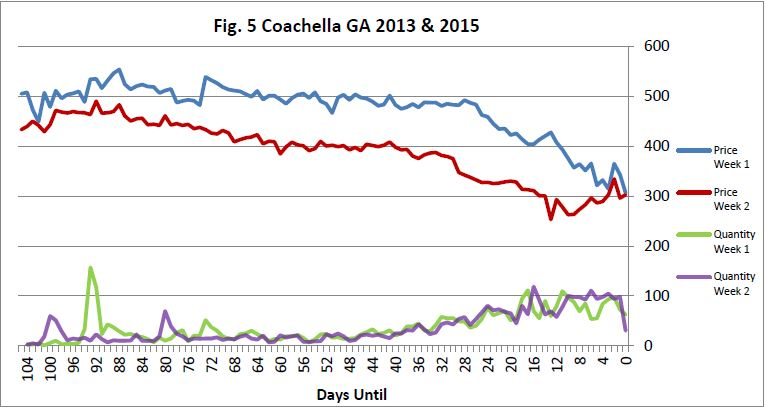
\includegraphics[width=0.68\textwidth]{chapter4/immagini/coachella1315}
	\caption{Vendite sui portali secondari delle edizioni 2013 e 2015 del Coachella Arts Festival}
	\label{coach}
\end{figure}
\begin{figure}[htbp]
	\centering
	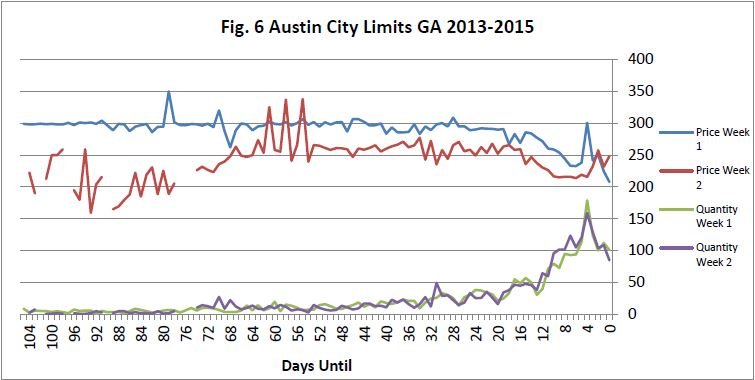
\includegraphics[width=0.68\textwidth]{chapter4/immagini/acl1315}
	\caption{Vendite sui portali secondari delle edizioni 2013 e 2015 di Austin City Limits}
	\label{acl}
\end{figure}
Si può notare come, con l'avvicinarsi dell'evento, da una parte sia aumentato il quantitativo delle vendite giornaliere, mentre dall'altra il prezzo medio sia progressivamente calato, a testimonianza della tesi sostenuta precedentemente. 
La rivista \textit{Forbes} cita come esempio le date italiane di \textit{On The Run Tour pt. II} di \textit{Jay-Z} e \textit{Beyoncé}, tenutesi nel Luglio 2018 presso gli stadi San Siro di Milano e Olimpico di Roma, in cui alcuni biglietti sul mercato secondario erano acquistabili a prezzi inferiori a 10€, contro un valore di emissione superiore ai 50€, prezzo minimo per le date sopracitate (Figura \ref{jayz}):
\begin{figure}[H]
	\centering
	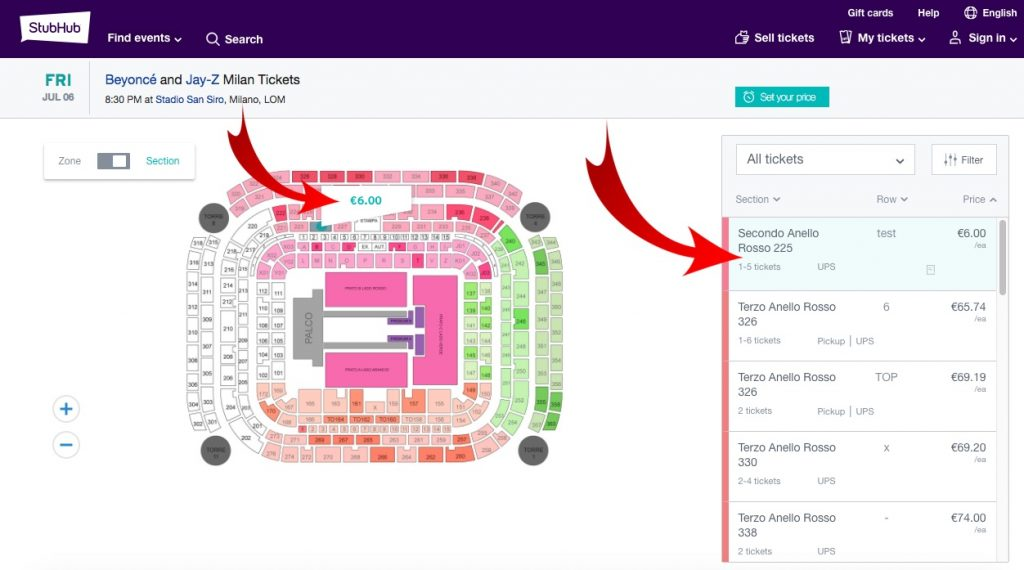
\includegraphics[width=0.68\textwidth]{chapter4/immagini/beyonce_jay_z}
	\caption{Biglietti per OTR II su StubHub}
	\label{jayz}
\end{figure}
La ragione di crolli sostanziali può avere tre spiegazioni logiche, basate anche sulle teorie espresse da Courty e Stein \cite{courty2014pricing, stein2014will}:
\begin{itemize}
\item Il biglietto aveva un Face Value sufficientemente alto e vicino al valore di mercato da lasciare gli speculatori con un quantità considerevole di biglietti invenduti da smaltire onde minimizzare le perdite e i costi di inventario.
\item Per gli eventi di grande portata i biglietti vengono emessi anche più di sei mesi in anticipo, e questo comporta un fisiologico flusso di rivendita nei giorni immediatamente precedenti. 
\item L'evento non ha venduto secondo le previsioni di mercato, e pertanto i biglietti sono reperibili sui portali dei rivenditori autorizzati. 
\end{itemize}
La volontà è quella di non lasciare utenti realmente bisognosi e desiderosi di privarsi del biglietto per impossibilità a partecipare con costi di inventario da sostenere e, al contempo, di contrastare le vendite di biglietti contraffatti sui portali secondari, fenomeno frequente soprattutto in casi di eventi di grossa portata \cite{phdthesis}.
%\section{Termini e Condizioni del Servizio}
\section{Tecnologie e piattaforme di sviluppo adottate} \label{sec:techno}
Equiticket è costruito su un'architettura Cloud di server dinamicamente scalabili di proprietà di \textit{Digital Ocean}: l'allocazione real-time di capacità computazionale relativamente al carico dell'applicazione garantisce le prestazioni richieste dagli utenti al minimo prezzo possibile.  
L'applicazione si serve inoltre di una logica proprietaria per la validazione dell'integrità del venditore e della transazione. Ad ora, Equiticket possiede anche un sistema CRM (Customer Relationship Management) in cui gli organizzatori certificati possono listare i propri eventi o gli utenti possono segnalarne di nuovi, se non fossero noti al sistema. Gli eventi segnalati dagli utenti sono considerati "aperti", e richiedono una verifica di legittimità da parte di un amministratore. \\*
Al fine dell'implementazione della logica di gestione dei pagamenti e dei controlli antifrode, ci si serve delle API di \textit{Stripe}, azienda B2B leader nella gestione di flussi monetari delle aziende e nello sviluppo di meccanismi di pagamento per siti di e-commerce. 
\subsection{PHP e Laravel}
Il portale Equiticket si presenta come applicazione server scritta in PHP avvalendosi del framework Laravel, pensato per il pattern architetturale di tipo Model-View-Controller (\textit{MVC}).
Laravel permette di specificare delle "rotte" (\textit{routes}), ovvero delle mappature univoche tra URL e le funzionalità offerte dall'applicazione. 
Laravel offre inoltre la possibilità di creare dei \textit{Controller}, allocati di default nella cartella "app/Http/Controllers". Ciascuno di questi Controller estende una classe e definisce comportamenti predefiniti in risposta a determinate azioni. Verranno ora esaminate singolarmente le tre componenti del pattern MVC in modo da mostrarne la struttura e le logiche architetturali. 
\subsection{Architettura Cloud dell'applicazione}
L'applicazione Equiticket risiede attualmente su server di proprietà di \textit{Digital Ocean}, azienda attiva nell'ambito del Cloud Computing. In particolare, ci si avvale di un servizio a pagamento di nome \textit{Droplets}, che consiste nella creazione di macchine virtuali (\textit{VM}) configurabili in grado di ospitare l'applicazione. \\
Una volta selezionato il tipo di VM richiesta e le specifiche tecniche, è sufficiente avviarla e  installare l'applicazione server, senza ulteriori accorgimenti gestionali o costi nascosti. In particolare, Digital Ocean offre una tariffazione oraria o mensile per il servizio "fully managed" Droplets: è possibile pagare o una quota mensile o una tariffa oraria per l'uptime delle macchine virtuali. \'E inoltre importante evidenziare come il Service Level Agreement (\textit{SLA}) offra un uptime garantito del 99,99\%, in modo che il sistema non risenta di eventuali problemi a livello fisico delle macchine. 
\subsubsection{Capacità di calcolo automaticamente scalabile} \label{loadb}
Una volta configurata la capacità di calcolo della macchina virtuale richiesta, è possibile configurare il servizio di \textit{Load Balancer} offerti da Digital Ocean: si tratta di un oggetto in grado di ripartire equamente il carico dell'applicazione su un dato numero di macchine virtuali, in modo da garantire sempre un throughput alto. Tramite l'uso del software \textit{DOProxy} è inoltre possibile creare un ambiente in cui il numero delle VM (o Droplet) attive scala dinamicamente in maniera orizzontale in base al carico in ingresso. Si tratta di uno script Ruby compatibile coi Droplet che montano una versione di Ubuntu maggiore di 16.04 e hanno installato \textit{HAProxy}, software liberato per la gestione di bilanciatori di carico. %Autoscaling fatto con DO? 
La procedura seguita per creare un'architettura software in grado di scalare automaticamente e resiliente a picchi di carico è la seguente: 
\begin{enumerate}
\item Creazione di un bilanciatore di carico ("\emph{Load Balancer}") con HAProxy. 
\item Creazione di uno o più Droplet tramite API ufficiale gestita da Digital Ocean.
\item Collegamento del Droplet al bilanciatore.
\item Definizione di una logica per la gestione e la scalabilità dei Droplet tramite uno script DOProxy (Ruby). In questo passaggio è possibile stabilire dei criteri di traffico in base ai quali gestire le proprie macchine virtuali. 
\end{enumerate}
Il risultato finale è l'architettura mostrata in Figura \ref{arcloud}: 
\begin{figure}[htbp]
	\centering
	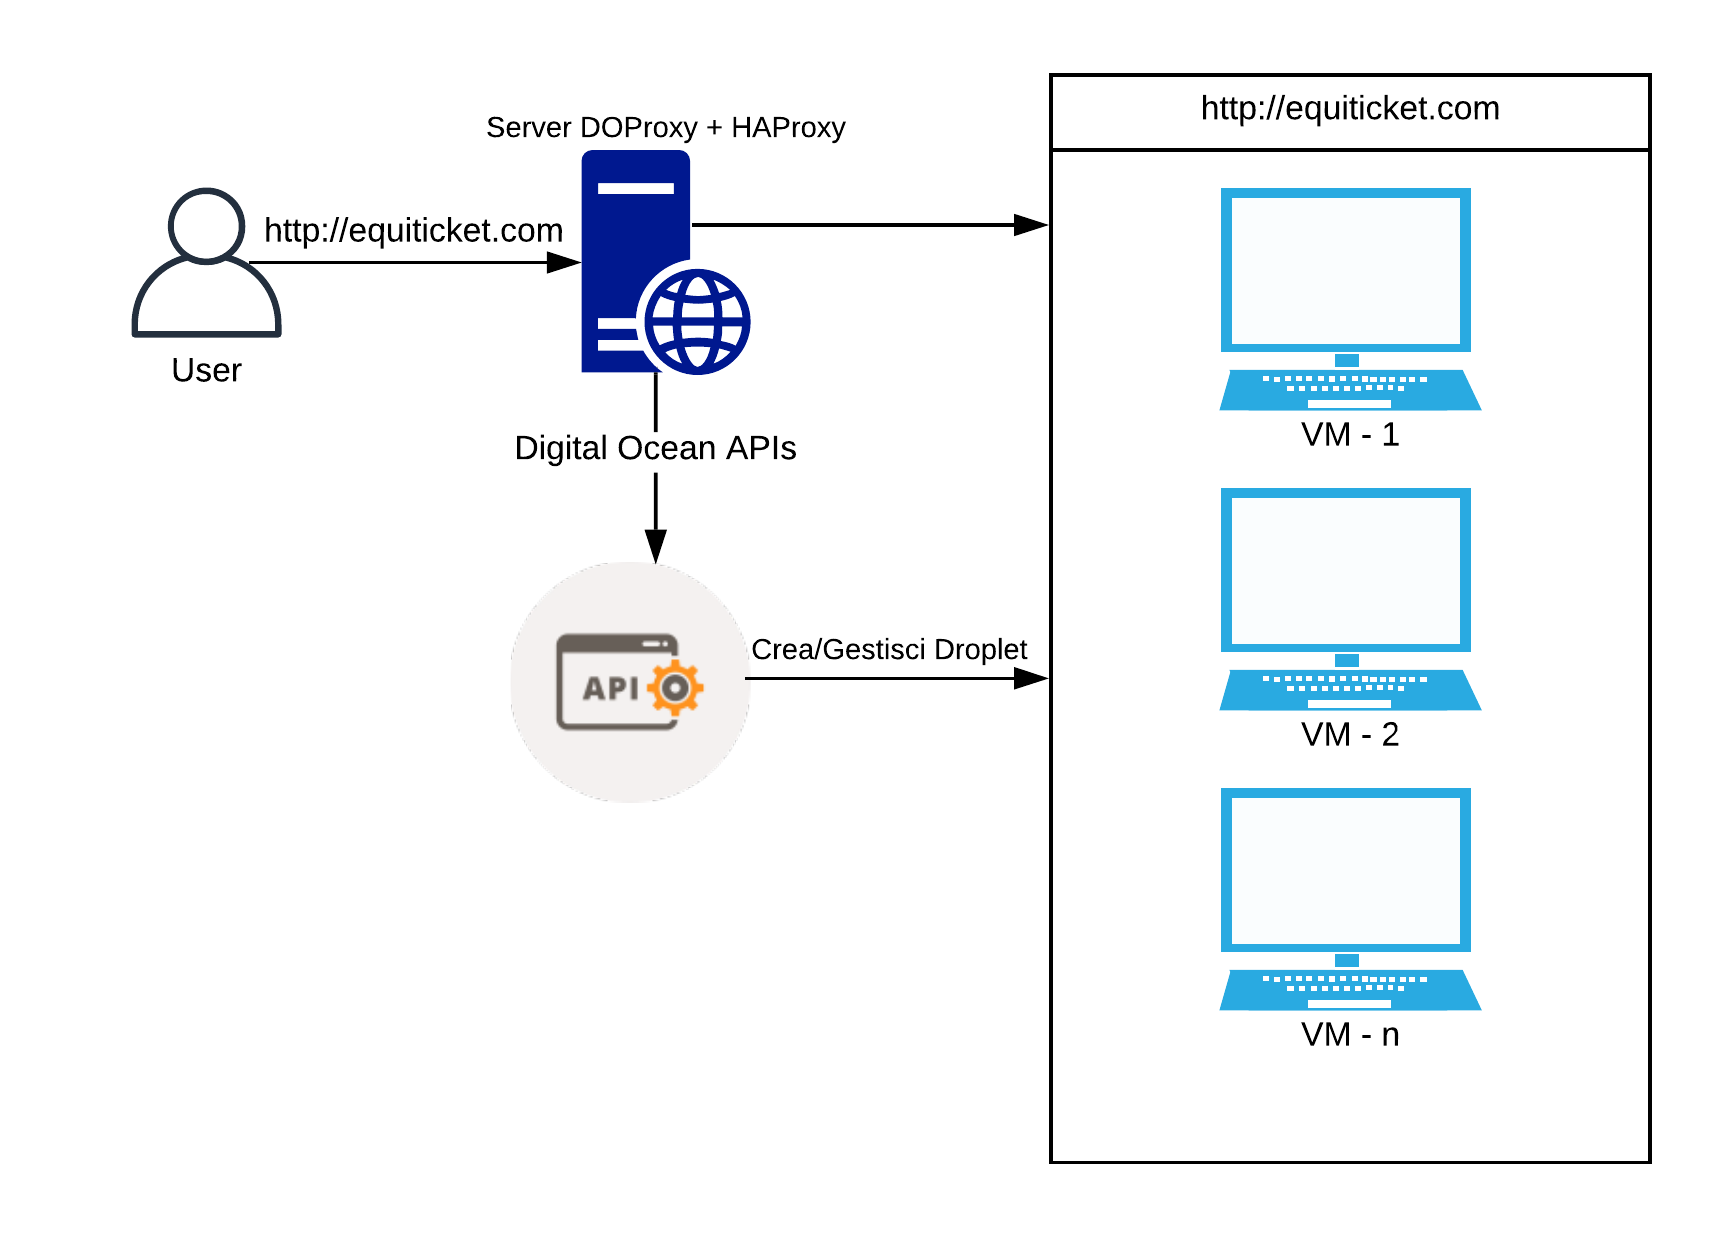
\includegraphics[width=0.68\textwidth, height=13cm, keepaspectratio]{chapter4/immagini/droplet}
	\caption{Architettura Cloud con \emph{Auto-Scaling} di Equiticket}
	\label{arcloud}
\end{figure}
\subsubsection{Vantaggi rispetto alla soluzione on-premise}
La soluzione Cloud presenta diversi vantaggi rispetto alla cosiddetta soluzione "on-premise", in quanto non sovviene la necessità di acquistare server e macchine fisiche: la capacità computazionale è infatti acquistabile da Digital Ocean secondo la formula "pay-as-you-go", sotto forma di macchine virtuali. Droplets è inoltre un servizio completamente gestito, in cui il titolare si fa carico della manutenzione delle macchine fisiche e del mantenimento dell'uptime stipulato sul Service Level Agreement. La scelta di una soluzione Cloud garantisce inoltre la possibilità di concentrarsi esclusivamente sull'attività del portale, sapendo che tutti i servizi complementari sono gestiti. 
\section{Requisiti funzionali e non-funzionali} \label{sec:requisiti}
% Architettura UML + Sequence Diagram?
\subsection{Design dell'interazione degli utenti}
Un'architettura ad alto livello delle interazione degli attori coi componenti del sistema Equiticket è descritta nella Figura \ref{usecase}:
\begin{figure}[htbp]
	\centering
	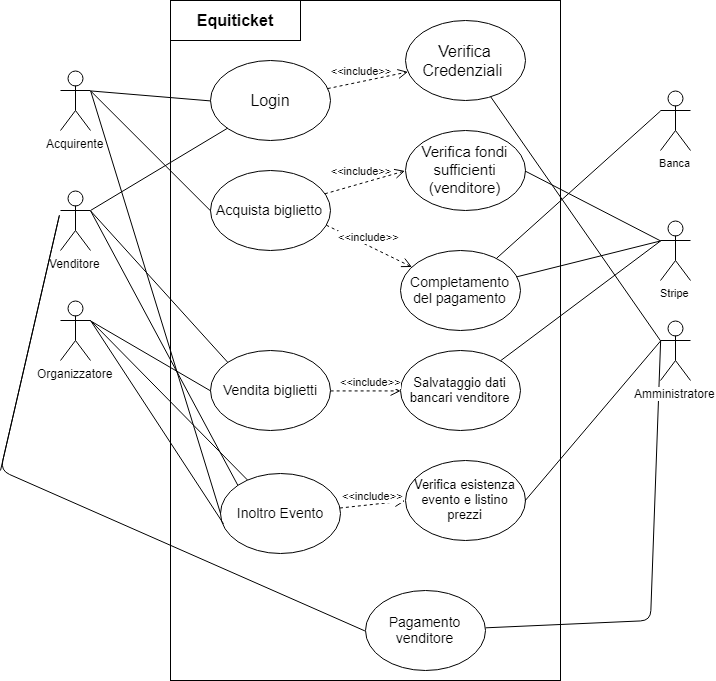
\includegraphics[width=0.68\textwidth]{chapter4/immagini/usecase}
	\caption{Use Case Diagram del portale Equiticket}
	\label{usecase}
\end{figure}
Gli attori principali individuati sono: 
\begin{itemize}
\item Acquirente (\textit{Customer}), utente registrato che può comprare titoli di accesso sul portale.
\item Venditore (\textit{Seller}), utente registrato in grado di poter mettere in vendita titoli di accesso sul portale.
\item Amministratore (\textit{Admin}), con accesso a tutti i dati di vendita, in grado di effettuare verifiche su nuovi eventi e, nel caso, inserirli a sistema.  
\item Organizzatore Eventi (\textit{Organizer}), che può listare i suoi eventi per la vendita di titoli di accesso.
\item \textit{Stripe}, i cui servizi vengono utilizzati attivamente in ogni tentativo di transazione. 
\end{itemize}
\subsubsection{Rivendita di un biglietto}
\textbf{\textit{Descrizione}}: L'utente registrato può mettere in vendita biglietti per un determinato evento. \\* 
Il portale effettua distinzione tra due tipi di eventi: 
\begin{itemize}
%TODO Template!
\item \textbf{Eventi \textit{"aperti"}}: eventi non presenti nel sistema, che hanno bisogno di una verifica di esistenza da parte di un Amministratore. Tali eventi possono essere segnalati da qualsiasi utente registrato al portale, ma non saranno pubblicati prima di una verifica dettagliata. 
\item \textbf{Eventi \textit{"chiusi"}}: eventi già presenti nella base di dati e la cui esistenza è già stata verificata. Di questi eventi sono noti anche tutti i valori di emissioni di tutte le tipologie di biglietto.
\end{itemize}
\textbf{\textit{Attori coinvolti}}: Utente registrato, Amministratore (facoltativo) \\*
\textbf{\textit{Pre-Condizione}}: L'utente deve essersi registrato al portale Equiticket fornendo i suoi dati e deve possedere il biglietto che desidera rivendere. \\*
\textbf{\textit{Azione}}: Se l'evento è chiuso, il sistema effettua un controllo sulla cifra richiesta dal venditore e controlla che sia minore o uguale al valore di emissione ufficiale. Se l'evento è aperto, il sistema lascia caricare il biglietto all'utente, e si riserva il diritto di approvarlo o respingerlo successivamente alle dovute verifiche. \\*
Il venditore può mettere in vendita due tipologie di biglietto: 
\begin{itemize}
\item Fisico, in formato cartaceo: in questo caso il venditore dovrà impegnarsi a recapitarlo all'acquirente entro sette giorni dalla vendita, come stabilito da \textit{Termini e Condizioni del Servizio} (o, più semplicemente, \textbf{\textit{T\&C}}). \'E possibile scegliere, al momento della messa in vendita, se la spedizione debba essere a carico del mittente o del destinatario.
\item Digitale, solitamente in formato PDF: in questo caso il venditore può caricarlo direttamente sul portale al momento della messa in vendita.
\end{itemize}
\textbf{\textit{Post-Condizione}}: L'utente carica con successo il biglietto sul portale per la rivendita. \\*
\textbf{\textit{Descrizione dettagliata del processo}}:
\begin{enumerate}
\item L'utente, previa registrazione, accede alla sua Area Riservata
\item Dopo aver selezionato l'opzione "Vendi biglietti", l'utente può selezionare un evento già esistente o inserirne uno. 
\item L'utente sceglie tipologia di biglietto e cifra richiesta, e può fornire una ricevuta d'acquisto.
%immagini del processo
\begin{figure}[htbp]
    \centering
    \begin{minipage}{0.45\textwidth}
        \centering
        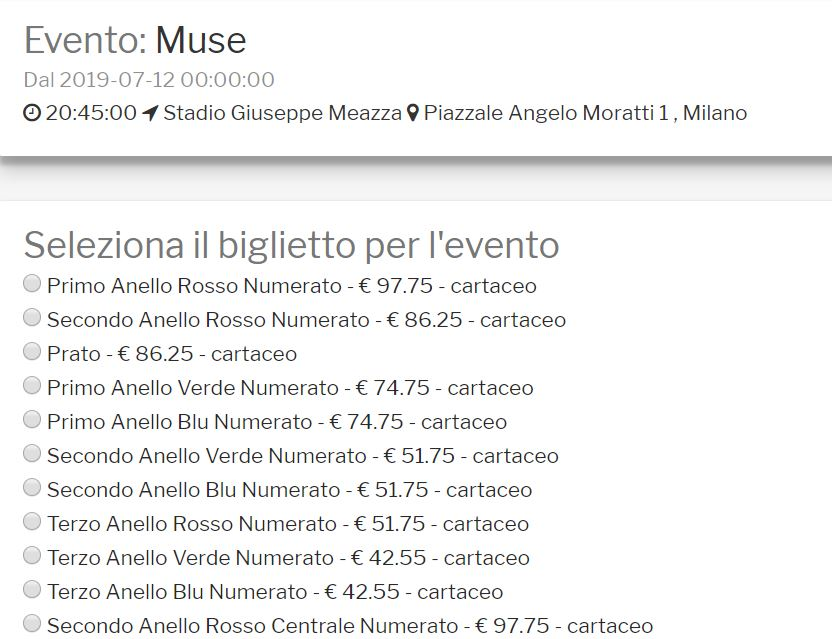
\includegraphics[width=0.9\textwidth]{chapter4/immagini/es_chiuso} % first figure itself
        \caption{Evento chiuso e noto al sistema}
				\label{evchiuso1}
    \end{minipage}\hfill
    \begin{minipage}{0.45\textwidth}
        \centering
        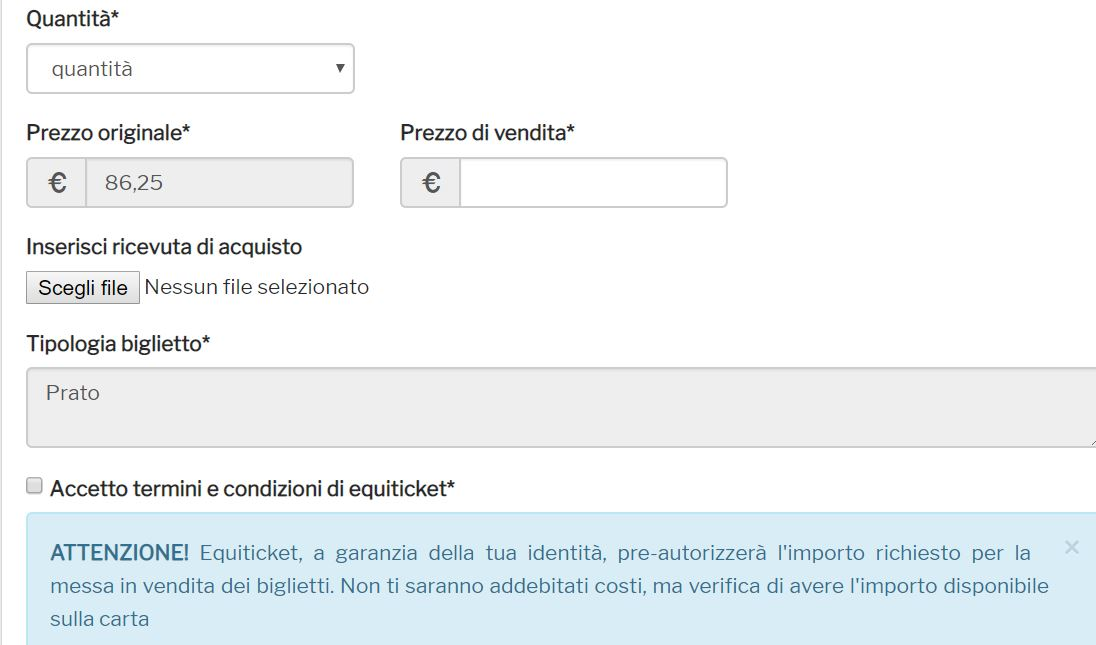
\includegraphics[width=0.9\textwidth]{chapter4/immagini/es_chiuso_2} % second figure itself
        \caption{Rivendita di biglietti per evento chiuso}
				\label{evchiuso2}
    \end{minipage}
\end{figure}
\begin{figure}[htbp]
    \centering
    \begin{minipage}{0.45\textwidth}
        \centering
        
\includegraphics[width=0.9\textwidth]{chapter4/immagini/ins_aperto} % first figure itself
        \caption{Possibilità di sottomissione di un evento}
				\label{evaperto1}
    \end{minipage}\hfill
    \begin{minipage}{0.45\textwidth}
        \centering
        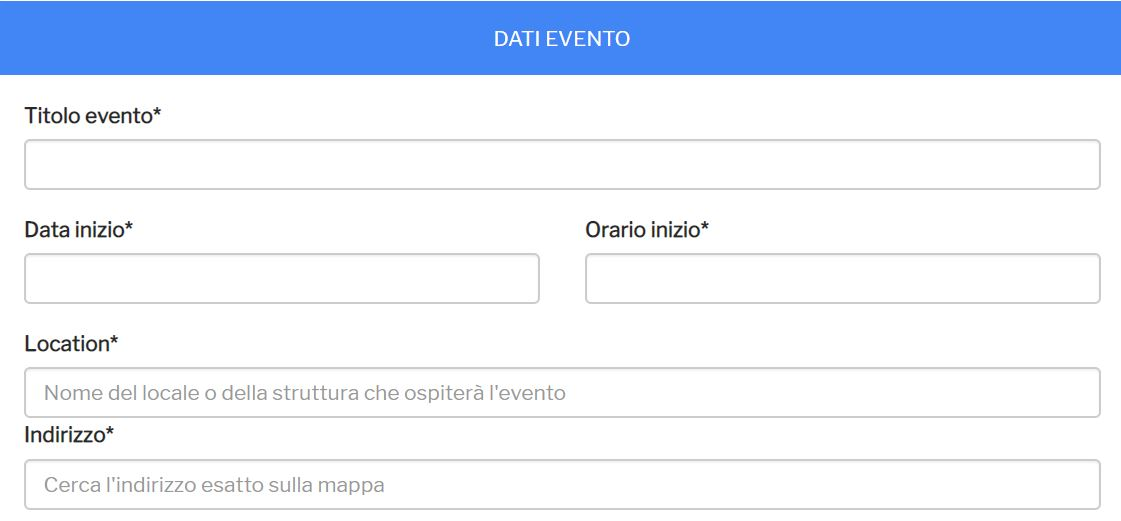
\includegraphics[width=0.9\textwidth]{chapter4/immagini/eventoaperto} % second figure itself
        \caption{Dati da fornire per la sottomissione}
				\label{evaperto2}
    \end{minipage}
\end{figure}
\item Una volta forniti tutti i dati dell'evento, vengono richiesti i dati della carta di credito al venditore, che verranno successivamente utilizzati da Stripe. 
\item Una chiamata API al metodo \textit{Authorization and Capture} di Stripe salva i dati della carta di credito del venditore in un oggetto chiamato \textit{Token}. Tale oggetto viene salvato su una base di dati proprietaria di Stripe, in modo che al portale non siano noti i dati sensibili bancari del cliente, come stabilito dalla normativa GDPR. \\* Al momento della cattura dei dati, non vengono effettuati né controlli su una eventuale disponibilità dei fondi, né pre-autorizzazioni per eventuali spese, né viene bloccata alcuna cifra: Stripe associa semplicemente i dati bancari del cliente a un Token univoco.
\item Il biglietto viene correttamente messo in vendita sul sito ed è disponibile per l'acquisto. Se l'utente ha inserito manualmente l'evento, tutto il processo necessiterà di un'approvazione manuale da parte di un Amministratore, che verrà notificato tramite e-mail al momento dell'avvenuta verifica.
\end{enumerate}
\textbf{\textit{Eccezioni ed errori gestiti}}:
\begin{itemize}
\item Il venditore richiede un prezzo superiore al valore di emissione del biglietto: in questo caso la vendita viene rifiutata e il venditore è invitato ad abbassare il prezzo.
\item Il venditore non fornisce i dati di una carta di credito (o prepagata) valida: in questo caso la vendita viene rifiutata, in quanto Stripe tramite le sue API è in grado di verificarne la legittimità con la Banca emittente. 
\end{itemize}
\paragraph{Stripe Token}
Il \textit{\textbf{Token}} è un oggetto monouso che cattura i dati di una data carta di credito, in modo che il sistema veda semplicemente un codice alfanumerico invece che i dati sensibili bancari del cliente. Il Token può essere utilizzato con due tipi di oggetto: 
\begin{itemize}
\item L'oggetto Charge, associato a un determinato addebito da eseguire sulla carta di credito corrispondente al Token.
\item L'oggetto Customer, al quale il Token può essere assegnato.
\end{itemize}
Si mostrano degli esempi di creazione e di applicazione del Token Stripe tramite frammenti di codice PHP: 
\begin{lstlisting}[language=PHP, caption={Creazione di un Token associato alla carta di credito indicata nell'array di nome card}]
\Stripe\Token::create([ \\
  'card' => [ \\
    'number' => '4242424242424242', \\
    'exp_month' => 6, \\
    'exp_year' => 2019, \\
    'cvc' => '101' \\
  ]
]);
\end{lstlisting}
\begin{lstlisting}[language=PHP, caption={creazione di un oggetto Customer, che verrà poi utilizzato per gestire pagamenti e vendite sul portale Equiticket}]
\Stripe\Customer::create([
  "description" => "Customer for a.pezzotta9@studenti.unibg.it",
  "source" => "tok_ubibanca" // obtained with Stripe.js
	// il codice del Token viene passato al costruttore dell'oggetto nella variabile "source"
]);
\end{lstlisting}

La descrizione del processo di rivendita di un titolo di accesso è descritta dal diagramma di sequenza in Figura \ref{seqacq}:
\begin{figure}[htbp]
	\centering
	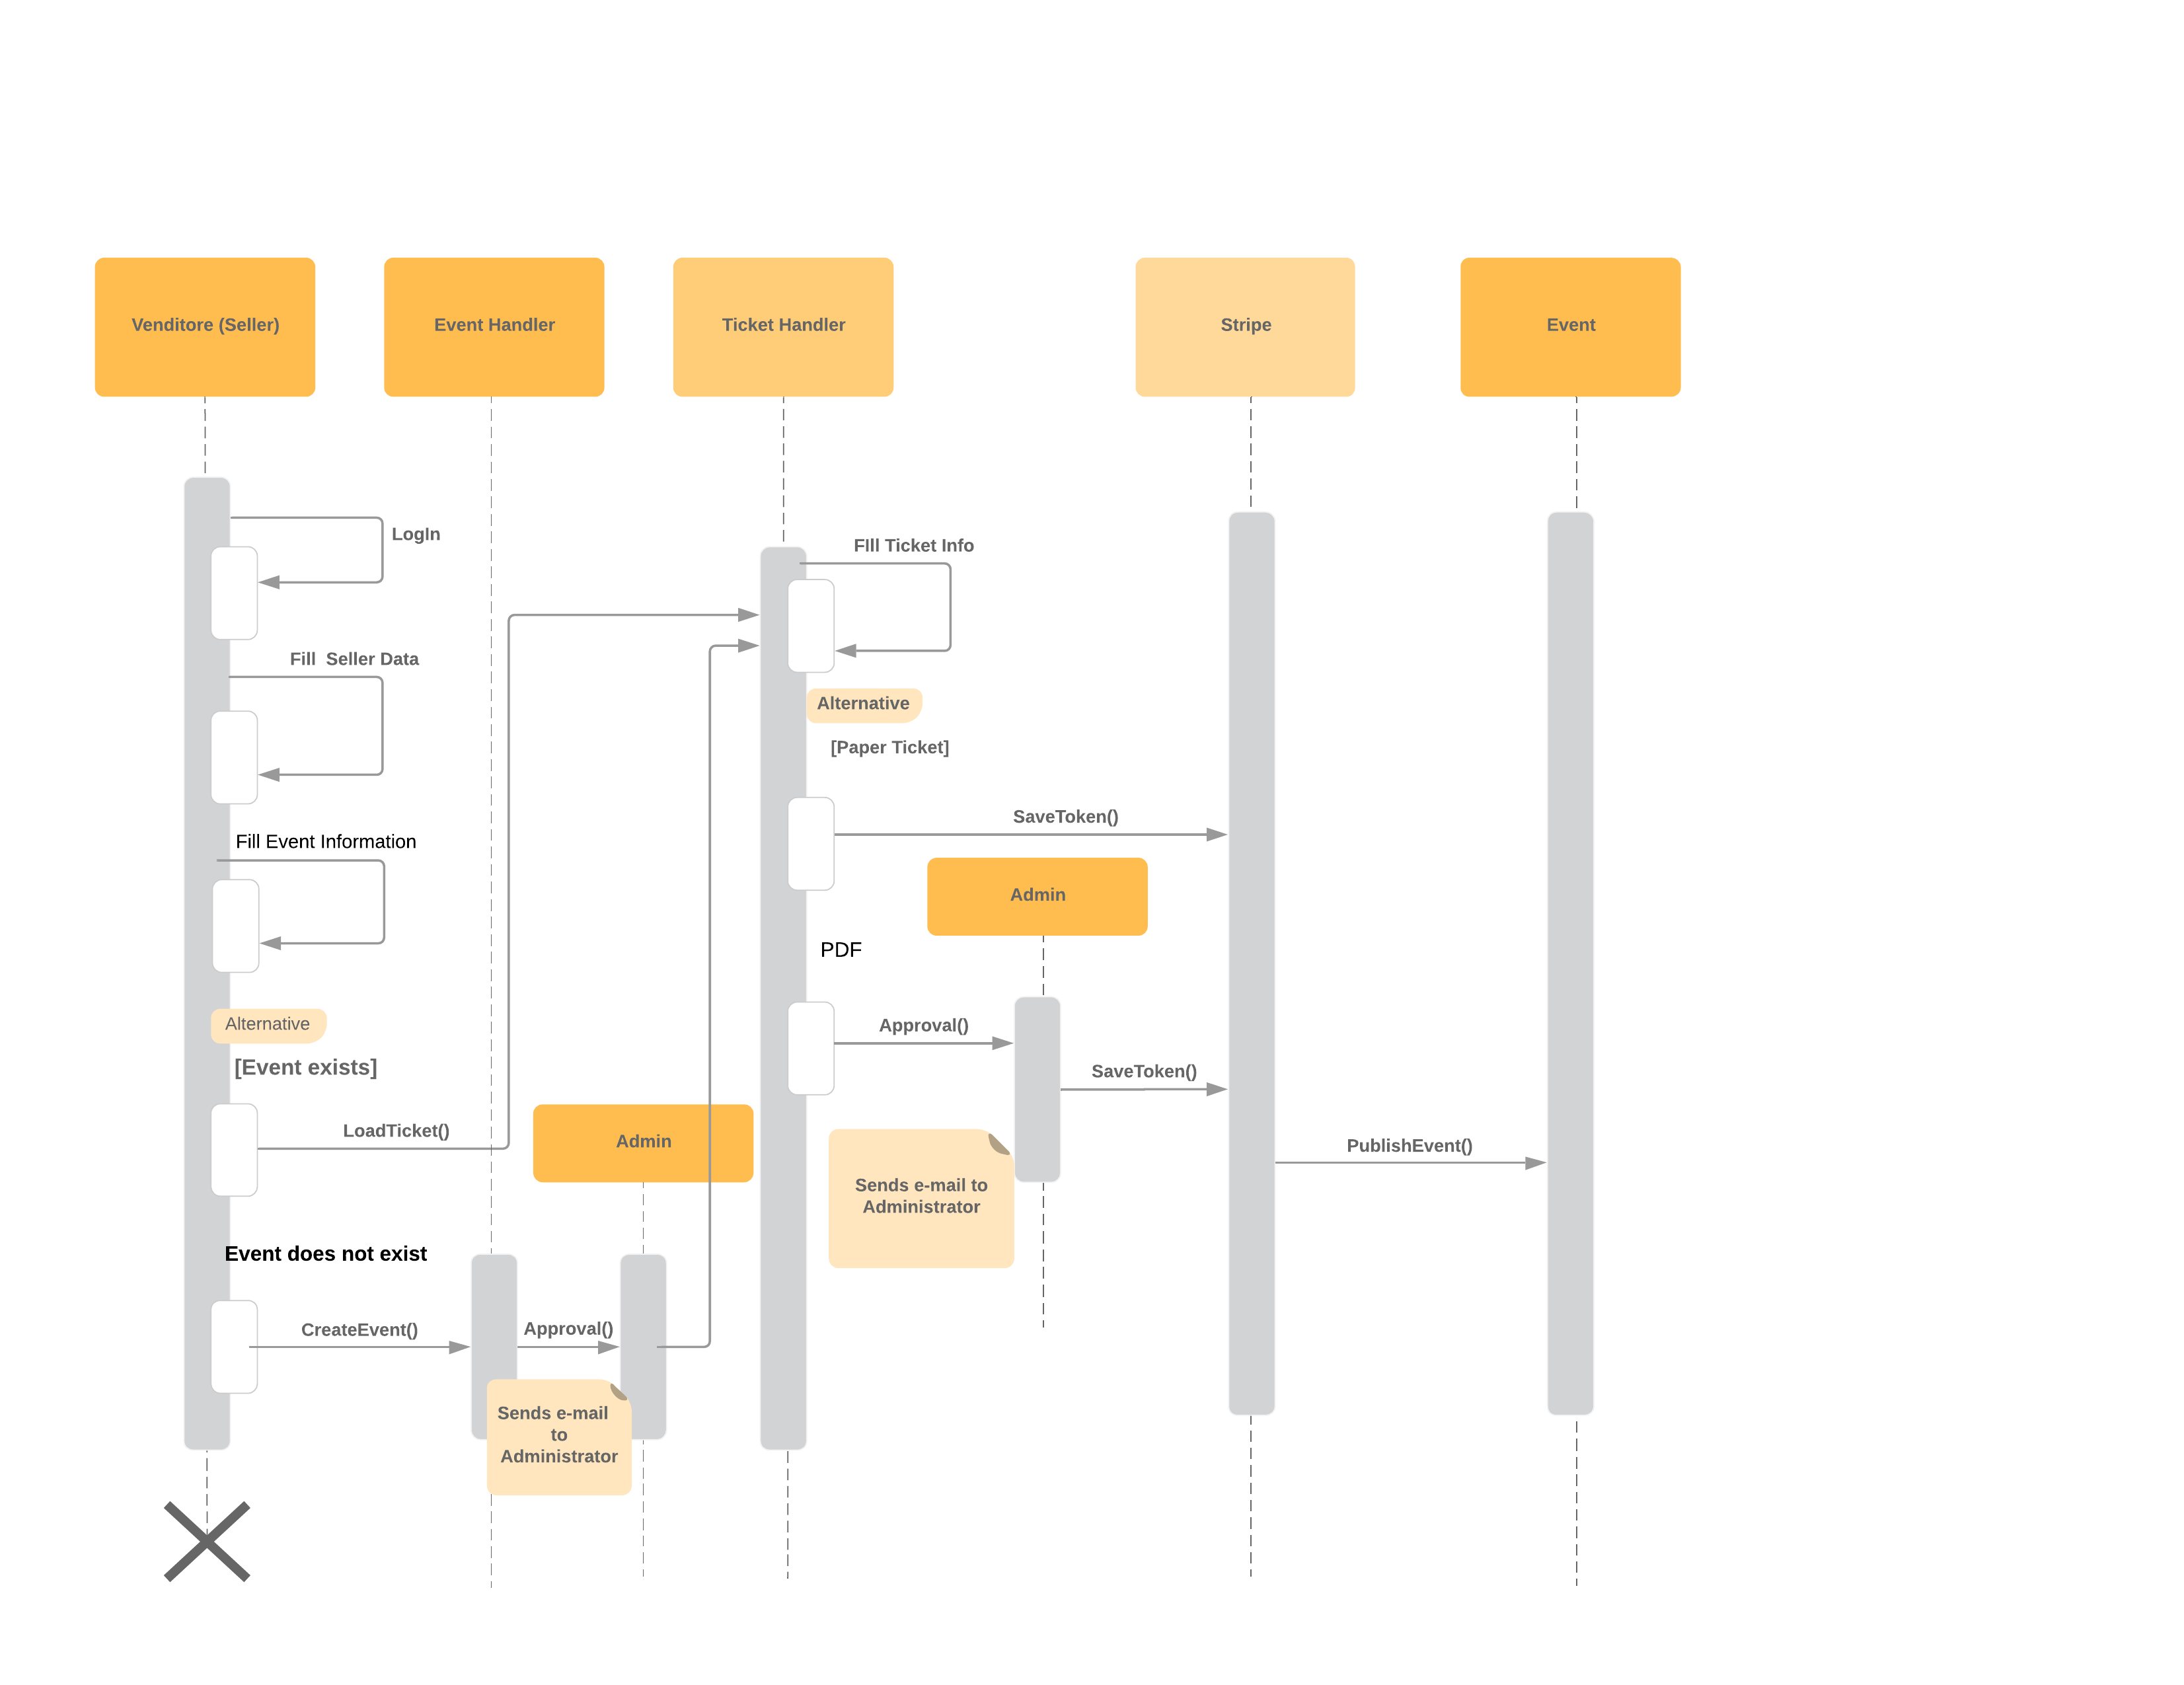
\includegraphics[width=\textwidth,height=\textheight, keepaspectratio, angle = 270]{chapter4/immagini/Rivendita}
	\caption{Diagramma di sequenza del processo di rivendita}
	\label{seqacq}
\end{figure} 
Dal diagramma emergono alcune ottimizzazioni a livello di struttura del processo che fanno in modo che l'esperienza di acquisto del cliente sia più rapida e piacevole possibile: il processo consta solamente di due pagine web, dopo le quali il biglietto sarà messo correttamente in vendita. Tra i più importanti accorgimenti sono annoverabili i seguenti: 
\begin{itemize}
\item Per l'utente, il processo da seguire è il medesimo, indipendentemente dal fatto che l'evento sia già esistente nel sistema oppure no: nel secondo caso la pubblicazione sul portale dipende dall'Amministratore del Sistema. 
\item Nel fornire le informazioni sul biglietto, il venditore può già scegliere la percentuale di sconto da applicare, il tipo di spedizione (e la persona incaricata del pagamento) e anche un possibile punto di ritiro per il corriere.
\item Il processo di approvazione dell'evento è trasparente all'utente, che non deve occuparsi di niente, se non di fornire i dati richiesti. 
\end{itemize}

\paragraph{Authorization and Capture}
\textbf{\textit{Authorization and Capture}} è una API di tipo POST sviluppata da Stripe, utilizzabile da aziende o privati per generare pre-autorizzazioni di pagamento e trattenere la cifra richiesta per un determinato lasso di tempo. \'E possibile creare un oggetto \textbf{\textit{Charge}} rappresentante l'addebito da effettuare sulla carta di credito dell'acquirente o del venditore. Tramite la tecnologia di Stripe è inoltre possibile decidere se la "cattura" del pagamento debba essere immediata o se semplicemente il pagamento vada pre-autorizzato. Una volta data la pre-autorizzazione, è possibile riscuotere il pagamento con garanzia della Banca coinvolta entro sette giorni. La natura del tipo di Charge va specificata al momento della creazione, aggiundendo al costruttore un parametro \textit{"capture"}: 
\begin{itemize}
\item Se questo parametro viene impostato a \textit{"\textbf{true}"} (come avviene di default nel caso non venga specificato \cite{stripedoc}), la Charge viene catturata immediatamente, e il denaro verrà scalato immediatamente dalla carta di credito del soggetto identificato dal Token. 
\item Se invece capture viene impostata a \textit{"\textbf{false}"}, il pagamento viene pre-autorizzato, e può essere riscosso entro sette giorni, con garanzia dell'istituto bancario che ha emesso la carta di credito in oggetto. Con questa soluzione, entro i sette giorni può essere addebitato anche l'utente rimuove tutti i dalla carta di credito o dal metodo di pagamento designato: in questo caso è la banca a coprire la quota lasciata scoperta dall'acquirente. 
\end{itemize}

\begin{lstlisting}[language=PHP, caption={creazione di un oggetto Charge, che verrà poi utilizzato catturare il pagamento corrispondente, con cattura immediata}]
\Stripe\Charge::create([
  "amount" => 2000,
  "currency" => "eur",
  "source" => "tok_ubibanca", 
  "description" => "Charge for a.pezzotta9@studenti.unibg.it",
	"capture" => "true" // valore di default, nel caso non venisse specificato
	// In questo caso, il pagamento sarebbe riscosso immediatamente
]);
\end{lstlisting}

\begin{lstlisting}[language=PHP, caption={creazione di un oggetto \textit{Charge}, che verrà poi utilizzato catturare il pagamento corrispondente, con cattura entro sette giorni}]
\Stripe\Charge::create([
  "amount" => 2000,
  "currency" => "eur",
  "source" => "tok_ubibanca", 
  "description" => "Charge for a.pezzotta9@studenti.unibg.it",
	"capture" => "false" // In questo caso, il pagamento viene solo pre-autorizzato
]);
\end{lstlisting}

\begin{lstlisting}[language=PHP, caption={cattura di un pagamento tramite le API Stripe}]
$ch = \Stripe\Charge::retrieve("ch_19yUdo2thesis2CQlMNMP5b"); //Token associato all'utente
$ch->capture();
// Il pagamento viene catturato immediatamente
\end{lstlisting}

\subparagraph{Pagamenti non catturati}
Secondo la documentazione delle API fornita da Stripe, i pagamenti non riscossi entro sette giorni scadranno e non saranno più catturabili. Bisognerà pertanto creare un nuovo oggetto Charge corrispondente al pagamento per poterlo processare nuovamente \cite{stripedoc}. Se si provasse a catturare un pagamento oltre dopo la scadenza della pre-autorizzazione, Stripe effettuerà un tentativo di addebito, ma in questo non ci sono garanzie: se l'utente rimuovesse i fondi dalla sua carta di credito, la Banca non coprirebbe la cifra scoperta. 
\subsubsection{Processo di acquisto} \label{acquisto}
\textbf{\textit{Descrizione}}: L'utente inserisce nel carrello il prodotto desiderato. Il sistema verifica la legittimità del venditore (tramite una chiamata API a un servizio di Stripe) e, nel caso positivo, permette l'acquisto tramite carta di credito. In caso contrario, il prodotto è rimosso dal carrello e dal sistema. \\*
\textbf{\textit{Attori coinvolti}}: Cliente, Venditore, Banca, Stripe \\*
\textbf{\textit{Pre-Condizione}}: Il controllo effettuato dalla API Stripe restituisce un risultato "true" \\*
\textbf{\textit{Trigger}}: L'utente inserisce il prodotto nel carrello. \\*
\textbf{\textit{Post-Condizione}}: L'utente acquista con successo il/i biglietto/i richiesto/i e il venditore viene pagato tramite bonifico bancario o PayPal. \\*
\textbf{\textit{Descrizione dettagliata del processo}}: 
\begin{enumerate}
\item L'utente inserisce il prodotto desiderato nel carrello
\item In seguito a un evento catturato da un metodo PHP, il sistema effettua una chiamata API al metodo "\textit{Authorization and Capture}", il quale verifica che il venditore del biglietto soddisfi i seguenti requisiti: 
\begin{enumerate}
\item La carta di credito sia ancora valida e non sia stata disattivata nel lasso di tempo successivo al primo controllo (effettuato al momento della messa in vendita).
\item La liquidità sulla sua carta di credito soddisfi la seguente equazione: 
\begin{align*}
\textbf{$ L = P_{t} + C_{s} + 50 $}
\end{align*}
dove $P_{t}$ rappresenta la cifra richiesta per il biglietto e $C_{s}$ il costo dell'eventuale spedizione tramite corriere. Si controlla inoltre che il venditore abbia una cifra superiore a $P_{t} + C_{s}$ di almeno 50€: questo importo è stato stimato essere il prezzo medio di un evento di intrattenimento in Italia. Tale cifra verrà detratta dal conto del venditore in caso questo tenti di truffare il compratore evitando di spedire il biglietto, oppure mettendone in vendita uno contraffatto o inesistente. Il portale Equiticket si impegna infatti a fornire all'acquirente un ticket valido nel caso in cui il venditore si sottragga ai doveri espressi nel contratto di T\&C.
\end{enumerate}
\item Se i requisiti sono soddisfatti, il consumatore può effettuare l'acquisto tramite carta di credito e terminare l'operazione. Al momento del pagamento (\textit{checkout}), l'utente pagherà un prezzo pari a: 
\begin{align*}
\textbf{$ P_{f} = K \cdot
{P_{t}} + C_{s} $}
\end{align*}
dove la cifra finale è data dai seguenti fattori: 
\begin{itemize}
\item $P_{t}$: cifra richiesta dal venditore. Tale importo dovrà essere positivo, ma minore del face value del biglietto originale. Tale condizione è esprimibile dalla seguente disuguaglianza: 
\begin{align*}
\textbf{$ 0 \leq{ P_{t}} \leq{ P_{fv}} $}
\end{align*}
\item $C_{s}$: costo della spedizione. Può essere nullo nel caso in cui la spedizione sia a carico del mittente o il biglietto sia in formato digitale: 
\begin{align*}
\textbf{$ C_{s} \geq{0} $}
\end{align*}
\item Il termine K rappresenta la commissione (\textit{"Transaction Fee"}) trattenuta dal portale, ed è un valore che non supera mai il 15\% del prezzo del biglietto sul portale: 
\begin{align*}
\textbf{$ 1 < K \leq{1.15} $}
\end{align*}
\end{itemize} 
\'E importante sottolineare che, in caso di spedizione di biglietto cartaceo, la API \textit{Authorization and Capture} trattenga la cifra richiesta sulla carta del venditore per sette giorni, intervallo di tempo stabilito da T\&C per spedire il biglietto. Entro questa fascia temporale, il venditore dovrà fornire il numero di tracking della spedizione effettuata.
Se invece si tratta di un biglietto digitale, la cifra viene rilasciata nel momento in cui l'acquirente effettua il download dalla sua area riservata. \\*
Dal punto di vista tecnico, queste due operazioni sono il risultato di tre chiamate API: 
\begin{itemize}
\item la API "Authorization and Capture" viene chiamata usando come parametri il token assegnato al venditore, il valore della cifra da trattenere e il booleano \textit{capture}, che in questo caso dovrà essere "true".
\item la API "Authorization and Capture" viene anche usata per generare la richiesta di addebito sulla carta di credito dell'acquirente: in questo caso non è necessario specificare il parametro "capture". Questa API viene anche usata nel caso in cui il venditore non spedisca il biglietto e debba quindi risarcire il cliente. 
\item la API \textit{Refund} viene chiamata in automatico quando scadono i sette giorni previsti da T\&C e il venditore conferma la spedizione. La cifra trattenuta sulla carta viene così rilasciata.
\end{itemize}
\item Alla fine del processo di acquisto, il venditore viene pagato con la modalità di pagamento selezionata. Il pagamento viene erogato una volta decorsi sette giorni dalla data dell'evento, finestra di tempo prevista da T\&C perché l'acquirente apra eventuali contestazioni (es. biglietti contraffatti o differenti da quelli richiesti)
\end{enumerate}
\textbf{\textit{Eccezioni ed errori gestiti}}: 
\begin{itemize}
\item Il venditore non supera il controllo effettuato dalla API Stripe: in questo caso la vendita viene annullata e il biglietto rimosso dal portale. L'utente visualizzerà un messaggio di errore, mente il venditore riceverà una mail dettagliata riguardante il fallimento dell'esperienza di acquisto. 
\item La carta di credito del cliente non ha sufficienti fondi per l'acquisto del biglietto: l'acquisto fallisce e l'utente è invitato a cambiare metodo di pagamento o annullare l'operazione. 
\item Il venditore supera il controllo, ma il biglietto non viene recapitato all'acquirente nei sette giorni previsti dai \textit{Termini e Condizioni del Servizio}: in questo caso la cifra $P_{t} + C_{s} + 50$ viene detratta dalla carta del venditore, e il portale Equiticket si impegna a fornire all'Acquirente un biglietto equivalente a quello richiesto. 
\end{itemize}
La descrizione del processo di acquisto è data dal diagramma di sequenza illustrato in Figura \ref{seqpur}:
\begin{figure}[htbp]
	\centering
	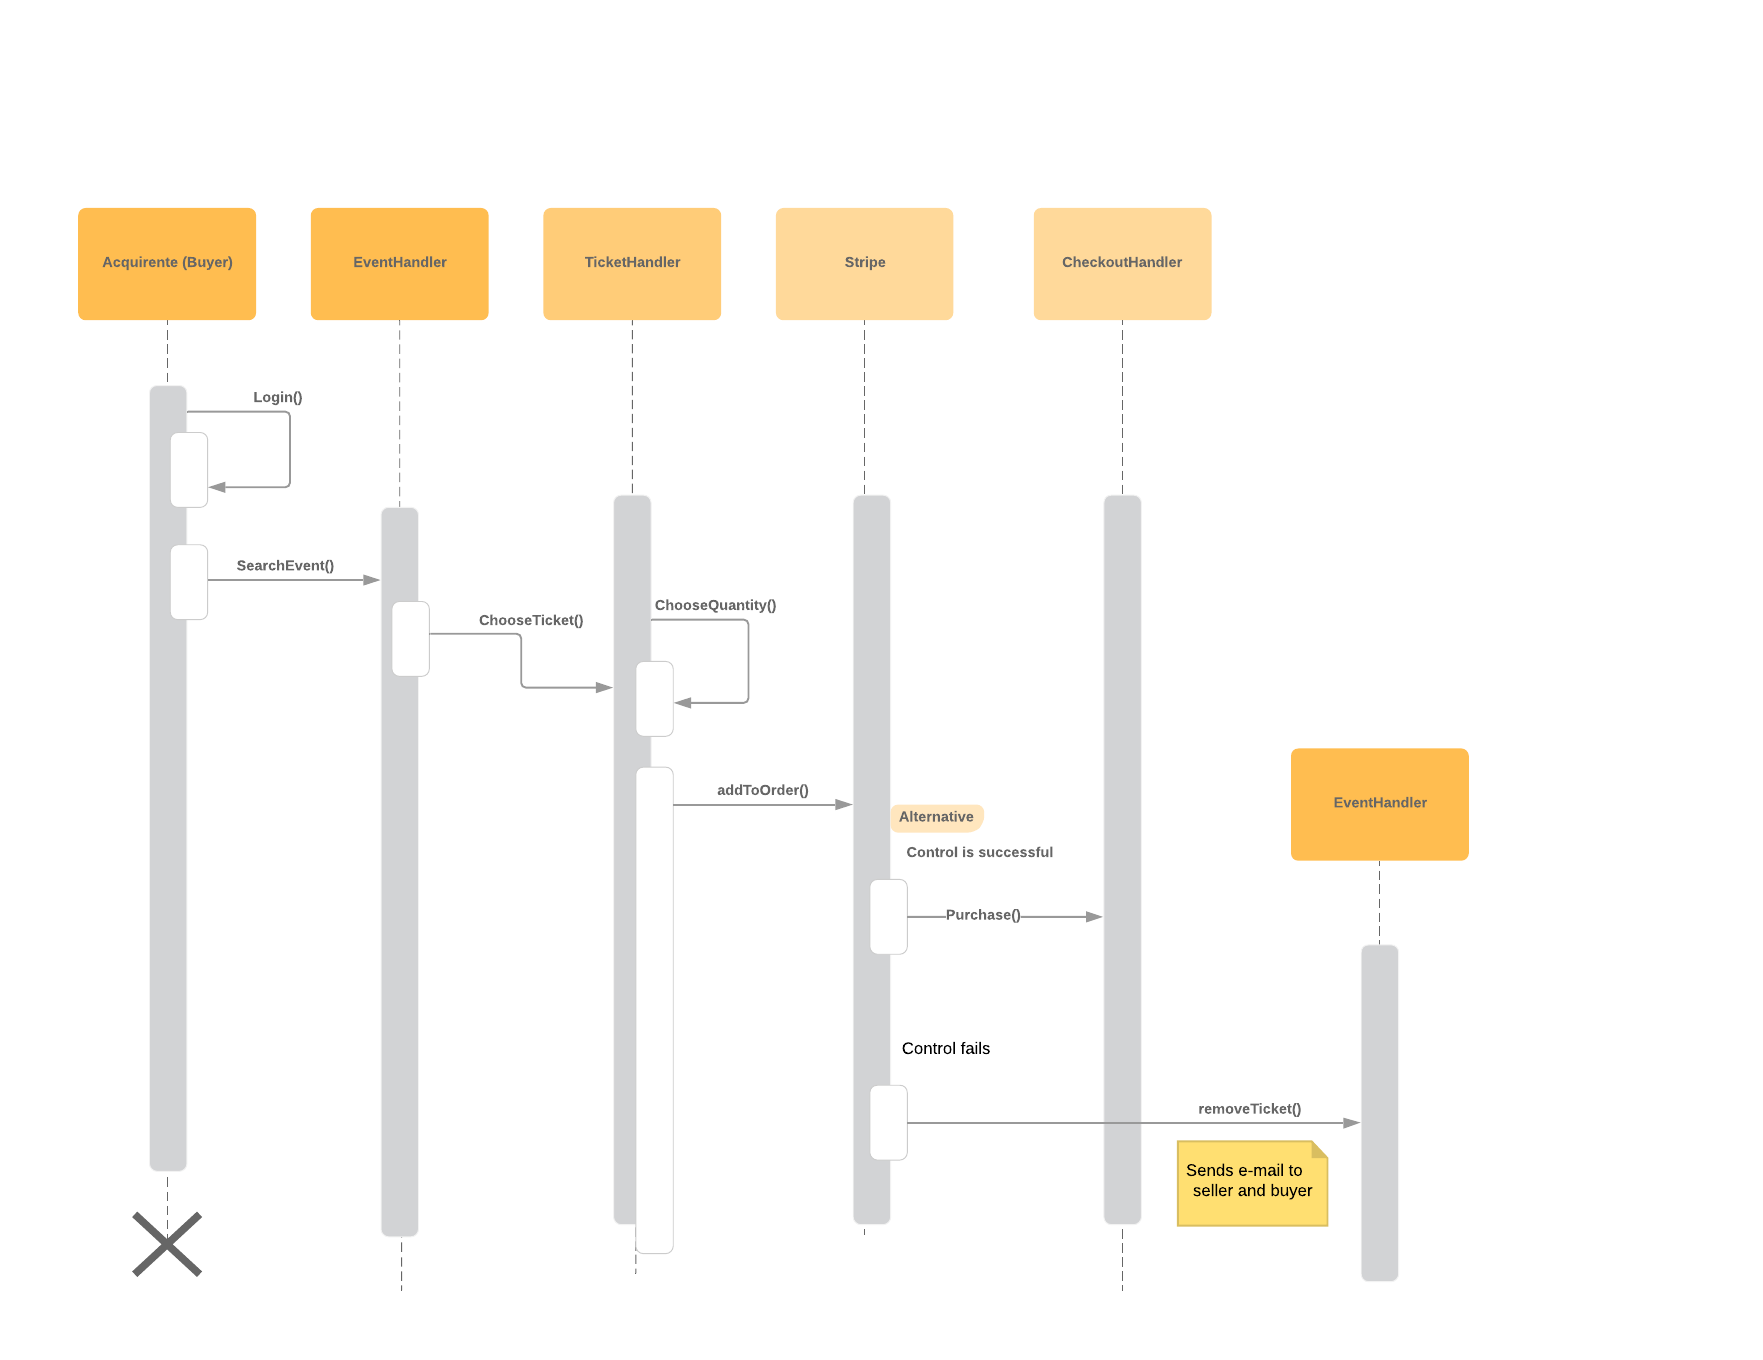
\includegraphics[width=\textwidth,height=\textheight, keepaspectratio, angle = 270]{chapter4/immagini/acquistoseq}
	\caption{Diagramma di sequenza del processo di rivendita}
	\label{seqpur}
\end{figure} 
Dal diagramma è possibile notare come l'acquirente possa acquistare il biglietto solo se il venditore supera i controlli di integrità precedentemente descritti. 
Viene ora illustrato un tentativo di acquisto, effettuato in data 11/03/2019, in cui il controllo antifrode entra in azione e blocca un potenziale acquisto pericoloso. 
Una volta scelto l'evento, è possibile, previa registrazione, selezionare un biglietto e inserirlo nel carrello, come mostra la Figura \ref{acq1}: 
\begin{figure}[htbp]
	\centering
	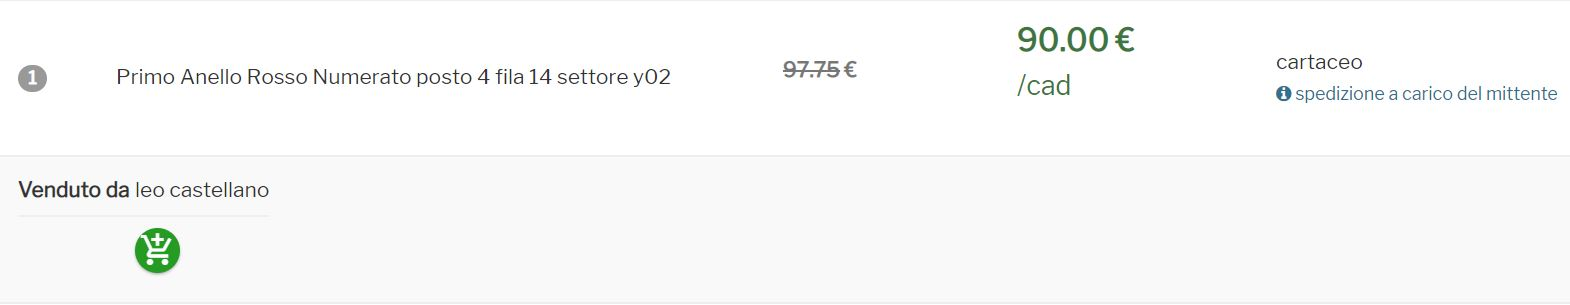
\includegraphics[width=0.68\textwidth]{chapter4/immagini/acquisto1}
	\caption{Scelta del biglietto per l'evento desiderato}
	\label{acq1}
\end{figure}
\begin{figure}[htbp]
	\centering
	
\includegraphics[width=0.68\textwidth]{chapter4/immagini/acquisto2}
	\caption{Inserimento nel carrello}
	\label{acq2}
\end{figure}
Appena inserito il biglietto nel carrello, la API \textit{Authorization and Capture} effettua il controllo sulla carta di credito fornita dal venditore. In questo caso, siccome i fondi non sono sufficienti, viene restituito un messaggio di errore all'acquirente (Figura \ref{fail1}):
\begin{figure}[htbp]
	\centering
	
\includegraphics[width=0.68\textwidth]{chapter4/immagini/acquisto3}
	\caption{Messaggio di errore: il venditore non ha fondi sufficienti}
	\label{fail1}
\end{figure} 
%Spedizioni

\subsubsection{Spedizione dei biglietti al destinatario}
\textbf{\textit{Descrizione}}: un acquirente ha acquistato con successo un biglietto dal portale Equiticket: questa sezione descrive in dettaglio come il titolo di accesso venga recapitato al legittimo destinatario. 
Come misura precauzionale, il sistema rimuove automaticamente tutti i biglietti per un dato evento quando mancano meno di quattro giorni alla manifestazione, nel caso si tratti di biglietti cartacei. \\*
\textbf{\textit{Attori coinvolti}}: Acquirente, Venditore, Corriere, Stripe, Banca (gli ultimi due sono facoltativi) \\
\textbf{\textit{Pre-Condizione}}: L'acquirente ha completato con successo il suo acquisto e attende la spedizione da parte del venditore. \\
\textbf{\textit{Azione}}: Il venditore, una volta completato il processo di vendita, deve provvedere alla spedizione (obbligatoriamente tracciata) entro una finestra temporale di sette giorni dal momento dell'acquisto. Si noti che, da contratto, la vendita è definitiva, e da questo momento non è possibile annullare il processo: il mancato adempimento dei propri doveri comporta la penale prevista da T\&C.\\
\textbf{\textit{Trigger}}: L'acquirente completa l'acquisto, pagando preventivamente anche le spese della spedizione (se previste) e le commissioni del portale Equiticket. \\
\textbf{\textit{Post-Condizione}}: L'acquirente riceve il biglietto in tempo utile per l'evento. \\
\textbf{\textit{Eccezioni ed errori gestiti}}: 
\begin{itemize}
	\item Il venditore non spedisce il biglietto in tempo utile: in questo caso la cifra $P_{t} + C_{s} + 50$,  descritta nelle sezioni precedenti, al momento trattenuta da Stripe, viene detratta dalla carta di 		credito del venditore, in modo che il portale Equiticket possa provvedere alla ricerca di un biglietto analogo a quello richiesto senza incorrere in ingenti perdite.
	Dal punto di vista tecnico, l'operazione di "cattura" di un pagamento precedentemente pre-autorizzato avviene tramite una chiamata API a Stripe, che agisce sull'oggetto \textit{Charge} assegnato al venditore. Alla chiamata è necessario soltanto il codice univoco del Token, che contiene già tutti i dati della cifra pre-autorizzata. 
	\item L'acquirente riceve un biglietto contraffatto: in questo caso ha sette giorni di tempo per aprire una contestazione sul portale Equiticket. Se le informazioni fossero vere, egli viene completamente rimborsato, mentre il venditore dovrà pagare una penale. 
	%spiegare meglio, parlare con Claudio!
\end{itemize}
\subsubsection{Inserimento di un evento}
\textbf{\textit{Descrizione}}: Un organizzatore o un utente registrato desiderano segnalare al sistema un evento non ancora presente nella base di dati: per farlo ricorrono all'apposita funzione presente nell'Area Riservata. \\
\textbf{\textit{Pre-Condizione}}: l'utente deve preventivamente essersi autenticato fornendo i suoi dati di accesso. \\
\textbf{\textit{Attori coinvolti}}: Organizzatore, Utente Registrato, Amministratore \\
\textbf{\textit{Azione}}: l'utente crea l'evento fornendo tutti i dati richiesti. L'Amministratore di sistema ha il compito, prima di pubblicare l'evento sul portale, di verificarne l'esistenza e i prezzi dei titoli di accesso. \\
\textbf{\textit{Trigger}}: L'utente sottomette la creazione di un evento. \\
\textbf{\textit{Post-Condizione}}: In seguito al controllo da parte di un Amministratore, l'evento viene pubblicato correttamente sul sito, e il portale Equiticket d'ora in poi potrà supportare le vendite dei biglietti per tale manifestazione. \\
\textbf{\textit{Eccezioni ed errori gestiti}}: 
\begin{itemize}
\item L'Amministratore non è in grado di verificare l'esistenza dell'evento, anche in seguito a ricerche: in questo caso l'evento non viene pubblicato e la richiesta dell'utente viene scartata. 
\end{itemize}
\textbf{\textit{Descrizione dettagliata del processo}}:
\begin{enumerate}
\item L'utente si registra sul portale, fornendo i suoi dati di accesso
\item L'utente clicca su "Crea evento" nella sua Area Riservata (Figura \ref{crea}):
\begin{figure}[htbp]
	\centering
	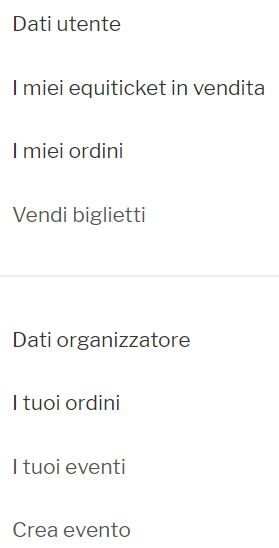
\includegraphics[width=0.68\textwidth, height=8cm]{chapter4/immagini/creaevento}
	\caption{Area riservata per creazione eventi}
	\label{crea}
\end{figure} 
\item L'utente fornisce i dati dell'evento compilando il form fornito dal portale (Figure \ref{form1} e \ref{form2}):
\begin{figure}[htbp]
    \centering		
    \begin{minipage}{0.45\textwidth}
        \centering
        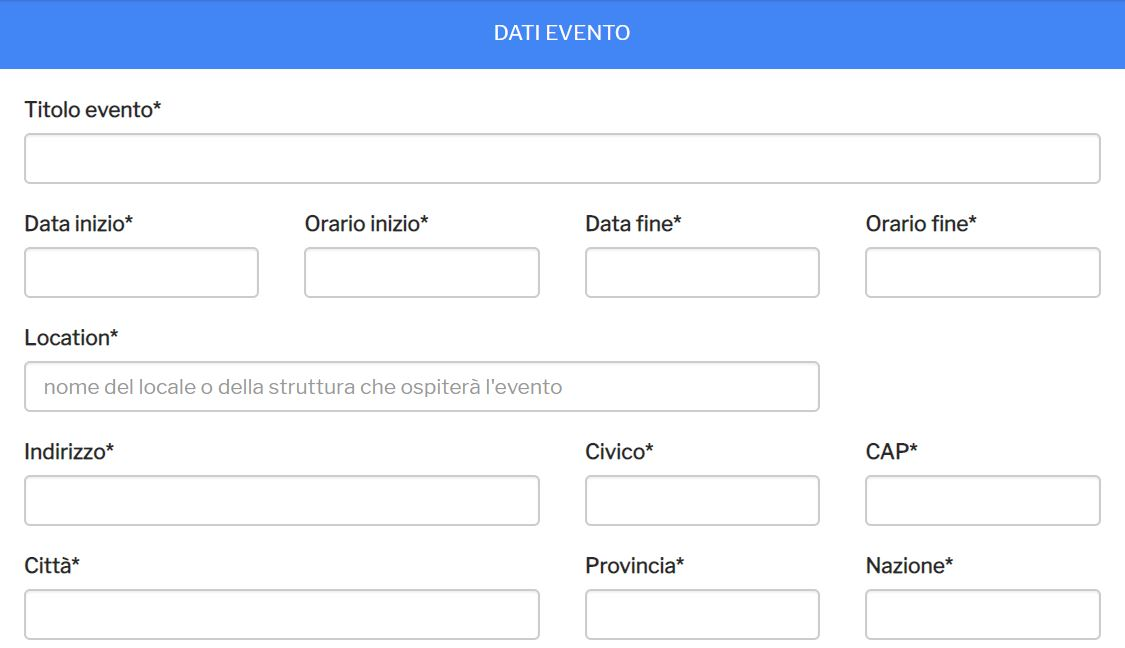
\includegraphics[width=0.9\textwidth]{chapter4/immagini/form1} % first figure itself
        \caption{Form, parte 1}
				\label{form1}
    \end{minipage}\hfill
    \begin{minipage}{0.45\textwidth}
        \centering				
        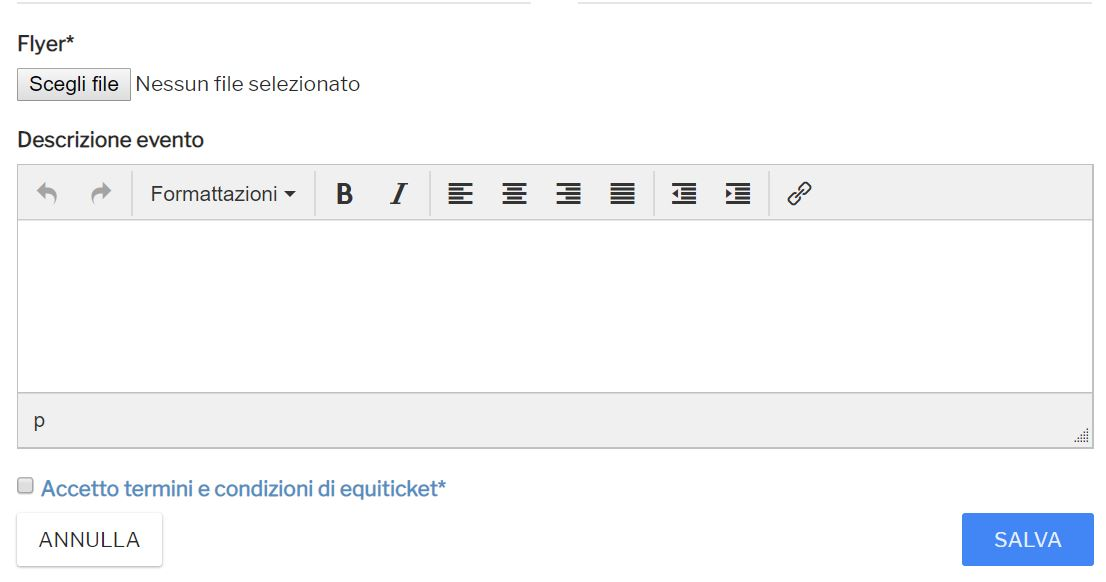
\includegraphics[width=0.9\textwidth]{chapter4/immagini/form2} % second figure itself
        \caption{Form, parte 2}
				\label{form2}
    \end{minipage}
\end{figure}
\item Una volta che l'utente sottomette la richiesta di creazione dell'evento, viene inviata una mail di notifica all'Amministratore del Sistema.
\item L'Amministratore verifica l'esistenza dell'evento e controlla i prezzi per l'acquisto dei biglietti. 
\item In base all'esito della ricerca, l'evento viene pubblicato sul sito, oppure la richiesta viene scartata. In caso positivo, d'ora in poi gli utenti e l'Organizzatore potranno vendere biglietti sul portale Equiticket. 
\end{enumerate}
\paragraph{Eventi e Template}
La gestione degli Eventi è fondamentale per il successo dell'applicazione Equiticket, e diventa di cruciale importanza avere un modello flessibile e facilmente utilizzabile per la creazione e la modifica di questi oggetti. Secondo la logica attuale, ogni evento approvato (chiuso) ha un suo \emph{\textbf{Template}}: esso consiste in un file XML che racchiude tutte le informazioni sull'evento creato. L'attuale motore PHP dell'applicazione è in grado di interpretarlo e visualizzarlo correttamente nella pagina web. \\
%Possibile immagine?
Oltre che per l'uso interno, i Template XML possono essere utilizzati anche in operazioni di comunicazione con siti esterni: ad esempio, i Template sono supportati da numerosi portali di annunci (in Italia sono molto noti, tra gli altri, \textit{Kijiji} e \textit{Subito}): risulta pertanto semplice la pubblicazione di un annuncio su portali esterni, nel caso in cui si volesse procedere a pubblicizzare in diverse maniere il prodotto. Grazie ai Template, la pubblicazione di un annuncio su un portale/servizio di terze parti si riduce alla chiamata di una API appartenente a terze parti. 
\section{Architettura software e implementazione} \label{sec:impl}
In questa sezione verranno descritti gli accorgimenti software utilizzati per implementare le misure di sicurezza descritti nelle sezioni precedenti. Il linguaggio utilizzato è il \emph{PHP}, che è stato scelto per lo sviluppo dell'applicazione. 
\subsection{Architettura a tre livelli}
L'applicazione consta di tre tipi di server, che seguono il paradigma della cosiddetta "\emph{Three-tiered architecture}" \cite{menasce2000scaling}: l'idea è quella di disporre tre strati di server, ognuno con una funziona diversa, in modo da poter ridirigere in maniera più efficiente le richieste effettuate dagli utenti. Il portale Equiticket si divide in: 
\begin{itemize}
\item \emph{Web Server}: lato dell'applicazione alla quale l'utente generico si interfaccia. Tutte le richieste effettuate vengono indirizzate al Web Server, il quale sfrutta le regole implementate dal Load Balancer descritto nella Sezione \ref{loadb}. 
\item	\emph{Application Server}: è il server in cui risiede tutta la logica business dell'applicazione e in cui vengono effettuate tutte le transazioni. 
\item \emph{Database Server}: Base di dati contenente i dati necessari per il funzionamento del portale, oltre a tutte le transazioni e i log dell'applicazione. 
\end{itemize}

%Immagine 3-Tier?
\subsection{Descrizione delle componenti}
\subsubsection{Modello}
\subsubsection{Vista}
\subsubsection{Controller}
\subsection{Gestione dei pagamenti e controllo anti-frode} \label{fraud}
%\Qui vanno tutti i frammenti di codice e le chiamate API
La logica che gestisce il controllo dei pagamenti e i controlli anti-frode si avvale di codice PHP proprietario unito ad alcune API fornite dall'azienda statunitense \emph{Stripe}. 
Il controllo effettuato dal sistema tramite Stripe si prefigge lo scopo di scongiurare i rischi di una possibile truffa per l'acquirente e garantire la migliore esperienza d'acquisto possibile. 
\subsubsection{Trattenute sulla carta di credito del venditore} \label{tratt}
Il controllo sulla carta di credito del venditore è necessario come garanzia, e si articola in più fasi: 
\begin{enumerate}
\item Quando il venditore mette in vendita il biglietto, deve inserire il numero della sua carta di credito. I dati verranno salvati su una base di dati di Stripe, mentre il portale Equiticket salverà semplicemente l'oggetto \textit{Token} generato dinamicamente da Stripe e associato univocamente all'utente.
%Codice authorizazion and capture Stripe per catturare i dati 
\item Quando l'acquirente inserisce il biglietto nel carrello, la API Authorization and Capture controlla che il venditore abbia fondi per la quantità $P_{t} + C_{s} + 50$, già descritta nella Sezione \ref{acquisto}
%Inserire frammento PHP => Got it!
\begin{lstlisting}[language=PHP, caption={Trattenuta della cifra $P_{t} + C_{s} + 50$ sulla carta del venditore quando l'acquirente inserisce il biglietto nel carrello}]
		$quantity = $request->get('quantity');
		$amount   = ((($equiticket->price_new + 50) * $quantity) + $equiticket->shipping_cost) * 100;

		if (!$equiticket->bypass_check){
			try {
				Stripe::setApiKey(env('STRIPE_SECRET'));

				$charge = \Stripe\Charge::create([
					'amount'   => $amount, // $15.00 this time
					'currency' => 'eur',
					'customer' => $equiticket->seller_card_id,
					'capture'  => false // l'importo viene soltanto trattenuto, non addebitato
				]);

			} catch(Card $exception) {
				$equiticket->accepted   = false;
				$equiticket->admin_note = $equiticket->admin_note . 'ATTENZIONE! biglietto sospeso in data ' . Carbon::now()->format('d-m-Y') . ' a causa di fondi insufficienti sulla carta di credito collegata.';
				$equiticket->save();
				Mail::to(env('MAIL_SYSTEM_TO'))->send(new NotifyNoFoundAvailableToAdmin($equiticket));
				Mail::to($equiticket->user->email)->send(new NotifyNoFoundAvailableToUser($equiticket));

				Session::flash('warning', 'equiticket selezionato non disponibile.');

				return redirect()->route('event.public-show', [$equiticket->event->id]);
			}

			$equiticket->seller_payment_uid = $charge->id;
		}

\end{lstlisting}
Dal codice, tratto dal metodo \textit{addToOrder}, si può notare che, se l'utente non ha i fondi necessari al momento del controllo effettuato dalla API Stripe (blocco TRY), viene lanciata l'eccezione del blocco CATCH, che genererà la notifica da mostrare a video all'utente e preparerà i template delle e-mail da inviare sia all'acquirente che al venditore. Tramite un metodo \textit{clearTicket}, il biglietto verrà rimosso dal sistema.
\item Quando l'acquirente acquista con successo il biglietto, viene richiamata la API Authorization and Capture, in cui stavolta il parametro "capture" viene passato come "true": così facendo, la cifra $P_{t} + C_{s} + 50$ viene trattenuta per un totale di sette giorni, finestra temporale in cui il venditore deve provvedere alla spedizione del biglietto secondo le modalità concordate.
%Inserire frammento PHP
\begin{lstlisting}[language=PHP, caption={Metodo \textit{checkout} per completare l'acquisto}]
try {
			Stripe::setApiKey(env('STRIPE_SECRET', 'sk_test_DgCFek4yzzfgLeHOr0xxO9h8'));

			$customer = Customer::create(array(
				'email'  => $request->get('stripeEmail'),
				'source' => $request->get('stripeToken')
			));

			$charge = Charge::create(array( //creazione della Charge da riscuotere
				'customer' => $customer->id,
				'amount'   => $order->total() * 100,
				'currency' => 'eur'
			));

			$order->user->buyer->update([
				'email'            => $request->get('email'),
				'telephone_number' => $request->get('telephone_number'),
				'address'          => $request->get('address'),
				'house_number'     => $request->get('house_number'),
				'postal_code'      => $request->get('postal_code'),
				'city'             => $request->get('city'),
				'province'         => $request->get('province'),
				'nation'           => $request->get('nation'),
				'society'          => $request->get('society'),
				'shipping_notes'   => $request->get('shipping_notes')
			]);

			$order->update([
				'email'            => $request->get('email'),
				'telephone_number' => $request->get('telephone_number'),
				'nation'           => $request->get('nation'),
				'total'            => $order->total(),
				'status'           => OrderStates::CLOSED,
				'payment_uid'      => $charge->id,
				'society'          => $request->get('society'),
				'shipping_notes'   => $request->get('shipping_notes')
			]);

			$order->updateBalance();

			$order->tickets->each(function (Ticket $ticket) use ($order) {
				for($i = 1; $i <= $ticket->pivot->quantity; $i ++) {
					$issue            = new TicketIssue();
					$issue->order_id  = $order->id;
					$issue->ticket_id = $ticket->id;
					$issue->unique_id = str_replace('.','',str_replace(' ','',microtime()));
					$issue->save();
				}
			});

			\Mail::to(env('MAIL_SYSTEM_TO'))->send(new ConfirmOrderToAdmin($order));
			\Mail::to($order->email)->send(new ConfirmOrderToUser($order));

			$order->equitickets->each(function (Equiticket $equiticket) use ($order) {
				\Mail::to($equiticket->user->seller->email)->send(new ConfirmEquiticketOrderToSeller($equiticket, $order));
			});
			$order->tickets->each(function (Ticket $ticket) use ($order) {
				\Mail::to($ticket->event->event_organizer->email)->send(new ConfirmTicketOrderToSeller($ticket, $order));
			});

			return view('cart.success');
		} catch(\Exception $ex) {
			return $ex->getMessage();
		}
	}
\end{lstlisting}
\item Una volta trascorsi sette giorni dalla data della trattenuta, oppure se l'acquirente rimuove il biglietto dal carrello, viene chiamata la API Refund di Stripe, che rilascia la cifra trattenuta sulla carta di credito del venditore, una volta avuta la conferma di spedizione.
%Inserire frammento PHP
\begin{lstlisting}[language=PHP, caption={Rilascio dei fondi sulla carta del venditore}]
if( ! $equiticket->bypass_check) {
			Stripe::setApiKey(env('STRIPE_SECRET'));
			$refund                         = \Stripe\Refund::create([
				'charge' => $equiticket->seller_payment_uid
			]);
			$equiticket->seller_payment_uid = null;
			$equiticket->save();
		}
\end{lstlisting}
\end{enumerate}
Solo in caso di mancata spedizione la cifra viene addebitata sul conto del venditore che non ha rispettato T\&C del servizio Equiticket.
% Inserire frammento PHP?
\section{Test della soluzione in casi reali} \label{sec:testing}
Questa sezione si occupa di mostrare il reale funzionamento del portale Equiticket: in particolare, verrà definito uno scenario di test in cui verranno simulate diverse situazioni, sia di tentata frode che di acquisto. Si vuole mostrare, sia dal punto di vista grafico che tecnico, tramite frammenti di codice, la risposta dell'architettura software a tali eventi. \\
Per il test dei casi d'uso e la verifica dell'effettivo funzionamento delle componenti descritte viene usata una metodologia di testing "\emph{black-box}": non si procederà con gli Unit Test delle classi e dei metodi, ma bensì si verificherà che il funzionamento effettivo sia uguale a quello descritto dai requisiti funzionali. Non si tiene conto della struttura implementativa degli oggetti nel corso di questi test, poiché si ritiene più importante concentrarsi sui criteri di rispetto dei requisiti. \\
I test vengono effettuati nell'ambiente di test di Equiticket: si tratta di un sito dedicato con il medesimo funzionamento del portale di produzione. Per un corretto svolgimento vengono usate le stesse API Stripe descritte in precedenza, con la differenza che la "Key" punterà all'ambiente di test e non a quello di produzione. La base di dati di riferimento è una copia ristretta di quella principale, in modo che i dati utilizzati non interferiscano con quelli reali che vengono trattati durante le transazioni. 
Tutti i test vengono effettuati in un ambiente dedicato, situato all'indirizzo "\emph{staging.equiticket.com}".
Gli attori coinvolti sono: 
\begin{itemize}
\item \textbf{\textit{Acquirente}}, simulato dal candidato con un'utenza personale.
\item \textbf{\textit{Venditore}}, simulato dal candidato con l'utenza istituzionale dell'Università di Bergamo.
\item \textit{\textbf{Amministratore}} di Sistema, con accesso a base di dati e log, simulato dal correlatore. L'Amministratore può accedere al pannello di controllo e avere visione completa di tutte le transazioni già avvenute sul portale e anche di quelle in corso, con relativi dettagli. Egli può inoltre modificare la tipologia degli eventi (aperti/chiusi) e approvare manualmente transazioni e contestazioni, se necessario. 
\item \textbf{\textit{Stripe}}: il corretto funzionamento delle logiche anti-truffa dipende dalle API utilizzate: per questo motivo si include il servizio come agente principale. Verranno usate due API sviluppate da Stripe e integrate nel codice sorgente di Equiticket: 
\begin{enumerate}
\item \emph{Authorization and Capture}, già descritta nel paragrafo dedicato, adibita alla pre-autorizzazione e alla cattura dei pagamenti pendenti. 
\item \emph{Refund}, utilizzata per il pagamento dei venditori e lo sblocco dei fondi trattenuti sulle carte di credito. 
\end{enumerate}
\end{itemize}
Per l'esecuzione dei test è stato scelto come evento la partita calcistica di Serie A Torino-Milan, e questo evento è inoltre stato contrassegnato come "aperto": in questo modo sarà possibile mostrare come queste manifestazioni necessitino di una ulteriore approvazione da parte di un Amministratore. 
Per garantire una maggiore coerenza dei risultati, si specifica che i test e i relativi screenshot sono stati effettuati tra il 18 e il 25 Aprile 2019. 

\subsection{Simulazione di un caso di tentata frode}
%TODO
In questo test, verrà simulata una frode in cui il venditore non supera il primo controllo effettuato sulla carta di credito, così che l'acquirente non possa acquistare con successo il biglietto: il biglietto verrà inoltre rimosso dal portale, in modo che nessun altro acquirente lo visualizzi come disponibile per l'acquisto. 
Il test viene così strutturato: 
\begin{enumerate}
\item Vengono create due utenze nell'ambiente di test, una adibita alla messa in vendita di un biglietto, l'altra all'acquisto. 
\item Viene messo in vendita un biglietto per un evento già esistente a sistema. Nel Token vengono salvati i dati di una carta di credito fasulla (\textit{Test Card}, \cite{stripedoc}) con un saldo inferiore alla cifra $P_{t} + C_{s} + 50$: 
\begin{equation}
S < P_{t} + C_{s} + 50
\end{equation}
Le Test Card sono delle carte di credito fittizie implementate da Stripe per i test di diversi casi d'uso: in particolare, la Test Card scelta permette l'associazione a un oggetto Customer e la creazione di un Token, ma non permette la creazione di alcuna Charge nei suoi confronti, pertanto ogni tentativo di addebito fallirà \cite{stripedoc} (Figura \ref{testvoid}).
\begin{figure}[htbp]
	\centering
	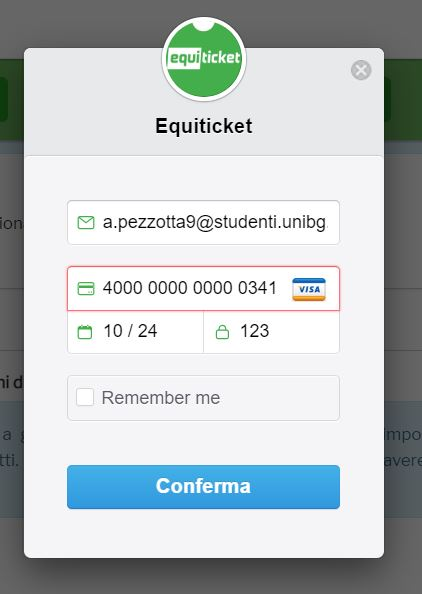
\includegraphics[width=0.68\textwidth, height=12cm]{chapter4/immagini/test2_cartavuota}
	\caption{Carta di credito non addebitabile}
	\label{testvoid}
\end{figure}
Tale operazione di cattura della carta di credito viene seguita chiamando la API Authorization and Capture descritta in precedenza: l'unica differenza è la "\emph{Stripe Key}", che in questo caso punterà all'ambiente di test.
\item Poiché si tratta di un \textit{evento aperto}, l'Amministratore deve approvarlo manualmente dal pannello dedicato (Figura \ref{testappr1} e \ref{testappr2}):
\begin{figure}[htbp]
	\centering
	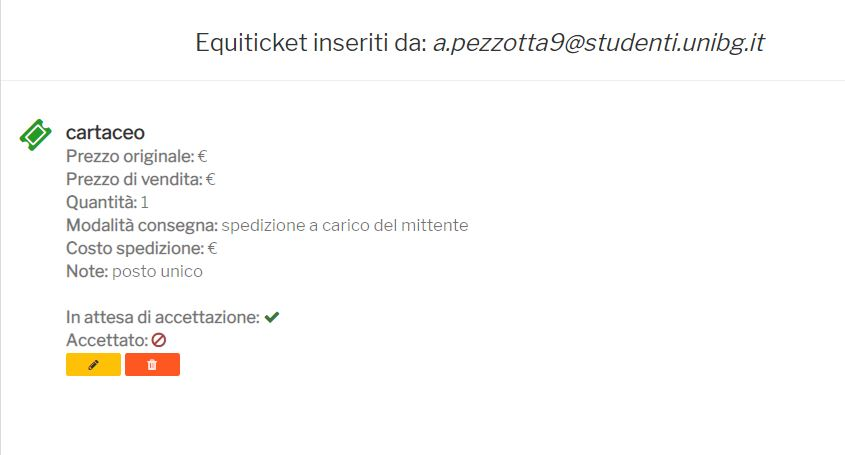
\includegraphics[width=0.68\textwidth]{chapter4/immagini/test_approvazione}
	\caption{Il biglietto appena sottomesso non è ancora approvato}
	\label{testappr1}
\end{figure}
L'Amministratore deve cliccare su "Accettato" e poi confermare la propria scelta perché il biglietto venga effettivamente messo in vendita: 
\begin{figure}[htbp]
	\centering
	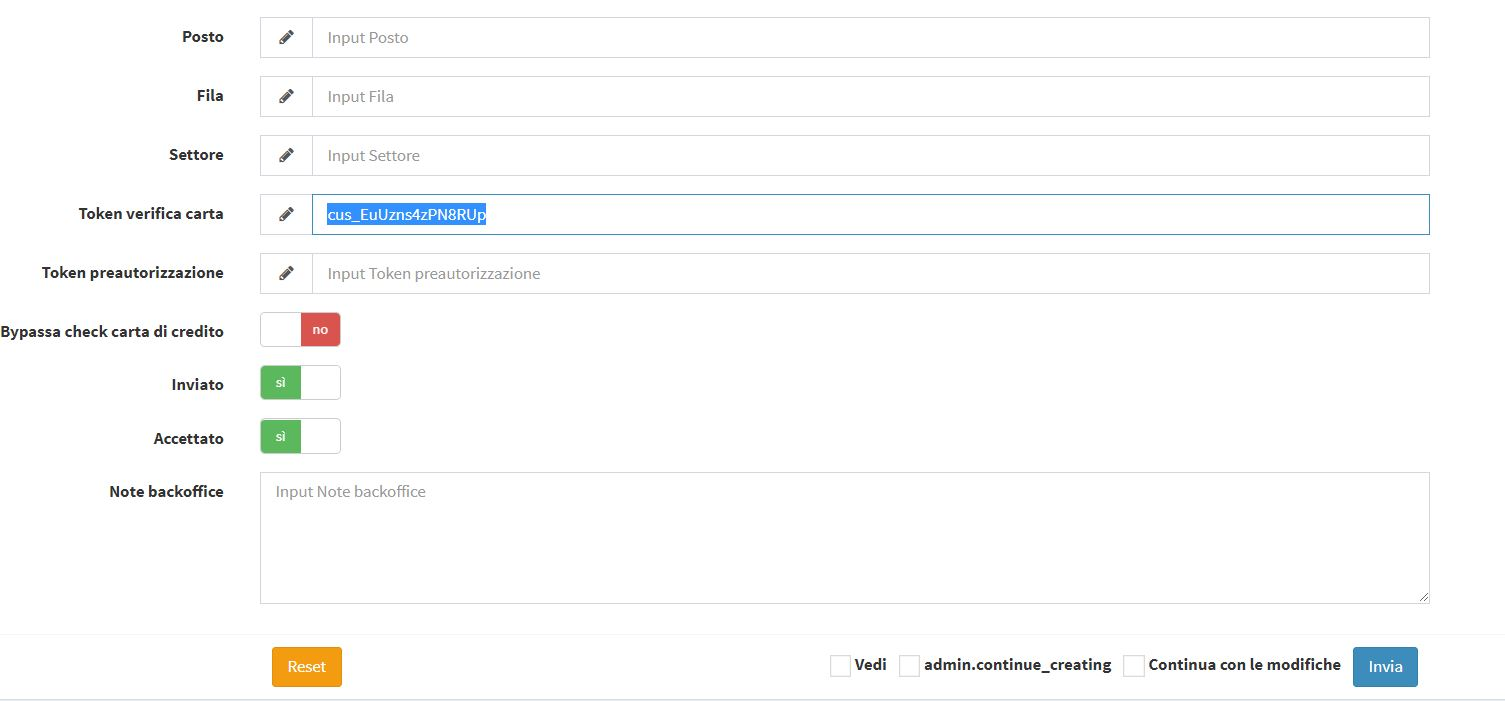
\includegraphics[width=0.68\textwidth]{chapter4/immagini/test_admin2}
	\caption{Approvazione dell'evento}
	\label{testappr2}
\end{figure}
Si ricorda che, se l'evento fosse stato già chiuso, questo step non sarebbe necessario, poiché in tal caso tutti i dettagli dell'evento sarebbero già noti al sistema. 
Una volta approvato (Figura \ref{accettato}), l'evento appare sul sito coi relativi biglietti in vendita: 
\begin{figure}[htbp]
	\centering
	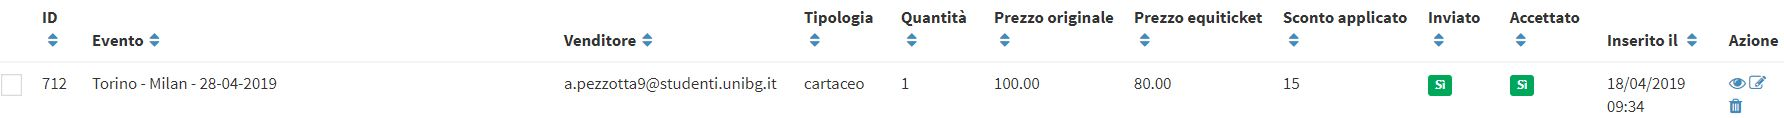
\includegraphics[width=0.68\textwidth]{chapter4/immagini/test_accettato}
	\caption{Evento post-approvazione}
	\label{accettato}
\end{figure}
\item L'acquirente inserisce nel carrello il biglietto in questione: il controllo di Stripe non rende possibile questa operazione in quanto la condizione del saldo disponibile non è soddisfatta. 
L'utente acquirente visualizza il seguente messaggio (Figura \ref{testfail1}): 
\begin{figure}[htbp]
	\centering
	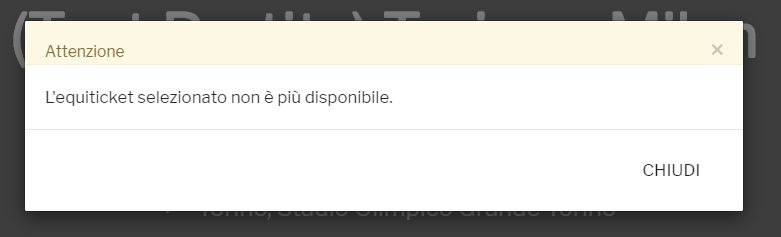
\includegraphics[width=0.68\textwidth]{chapter4/immagini/test2_nondisp}
	\caption{Biglietto non disponibile in seguito al fallimento del controllo Stripe}
	\label{testfail1}
\end{figure}
Il venditore riceve la seguente mail (Figura \ref{mailfail}), la quale segnala che il biglietto viene rimosso causa mancanza di fondi sulla carta di credito: 
\begin{figure}[htbp]
	\centering
	
\includegraphics[width=0.68\textwidth]{chapter4/immagini/mail_fail}
	\caption{Mail indicante il fallimento del controllo Stripe}
	\label{mailfail}
\end{figure}
\item L'acquirente non acquista il biglietto e il biglietto viene rimosso dal sistema. La rimozione del titolo di accesso dal portale è visibile dal pannello di amministrazione (Figura \ref{admfail}):
\begin{figure}[htbp]
	\centering
	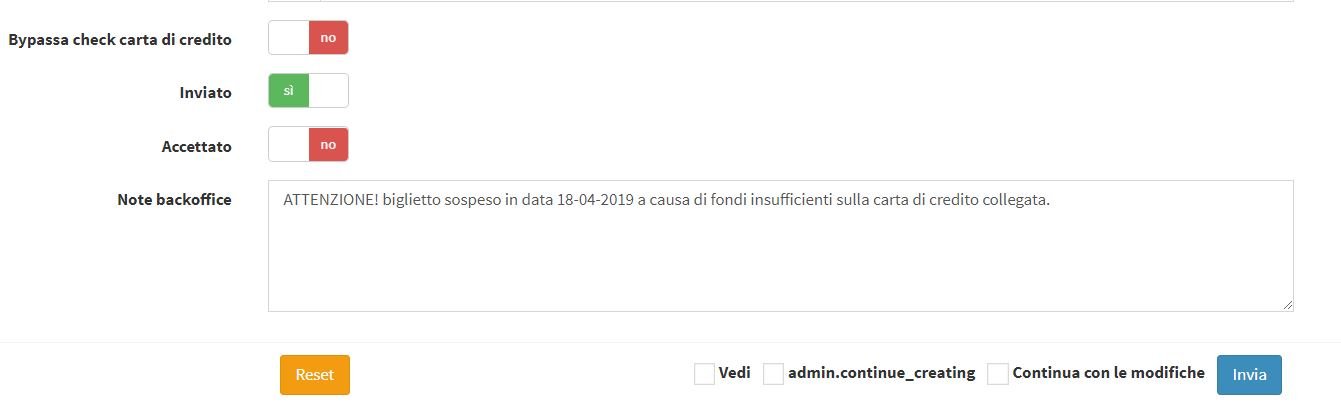
\includegraphics[width=0.68\textwidth]{chapter4/immagini/test2_fail2}
	\caption{Biglietto eliminato}
	\label{admfail}
\end{figure}
%simulare manualmente la mancata spedizione
\end{enumerate}

\subsection{Simulazione di una transazione terminata con successo}
In questo test verrà simulato uno scenario in cui un utente registrato mette in vendita un biglietto, un acquirente lo acquista e lo riceve entro i sette giorni prestabiliti da T\&C: in questo caso il venditore viene pagato da Equiticket sette giorni dopo che l'evento ha avuto luogo: nel corso di questa finestra temporale l'acquirente può aprire una contestazione nel caso in cui il biglietto ricevuto sia contraffatto o diverso da quello acquistato (es. posti a sedere diversi). 
Il test viene così strutturato: 
\begin{enumerate}
\item Viene messo in vendita un biglietto per un evento già esistente a sistema (evento chiuso). Nel Token (Figura \ref{testtok}) vengono salvati i dati di una carta di credito fasulla con un saldo superiore alla cifra $P_{t} + C_{s} + 50$ (Figura \ref{testev}): 
\begin{equation}
S \geq{P_{t} + C_{s} + 50}
\end{equation}
\begin{figure}[htbp]
	\centering
	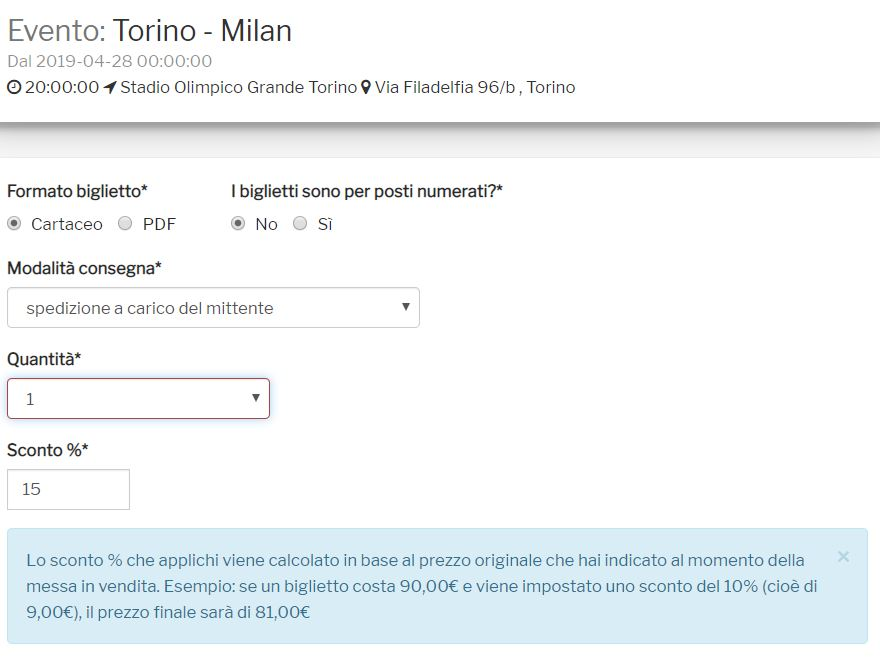
\includegraphics[width=0.68\textwidth]{chapter4/immagini/test_vendi}
	\caption{Evento scelto per il test}
	\label{testev}
\end{figure}
\begin{figure}[htbp]
	\centering
	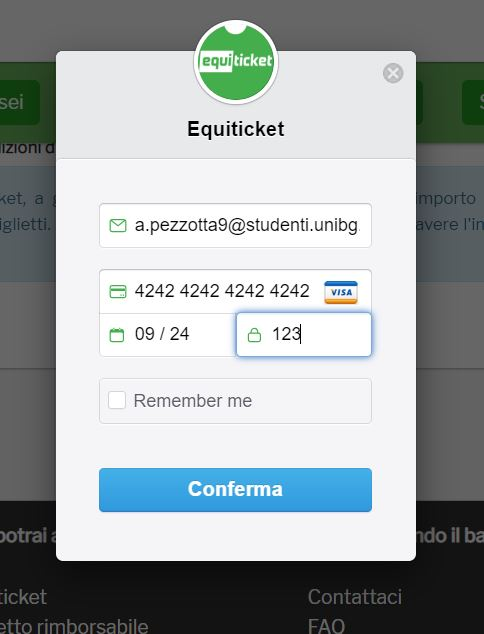
\includegraphics[width=0.68\textwidth]{chapter4/immagini/test_token}
	\caption{"Test card" utilizzata da Stripe per la creazione del Token}
	\label{testtok}
\end{figure}
La Test Card selezionata in particolare è una di quelle con fondi virtualmente illimitati, che può quindi acquistare per qualsiasi cifra e superare i controlli previsti dalla procedura di acquisto. 
\item L'acquirente inserisce il biglietto nel carrello e lo acquista con successo.
\begin{figure}[htbp]
	\centering
	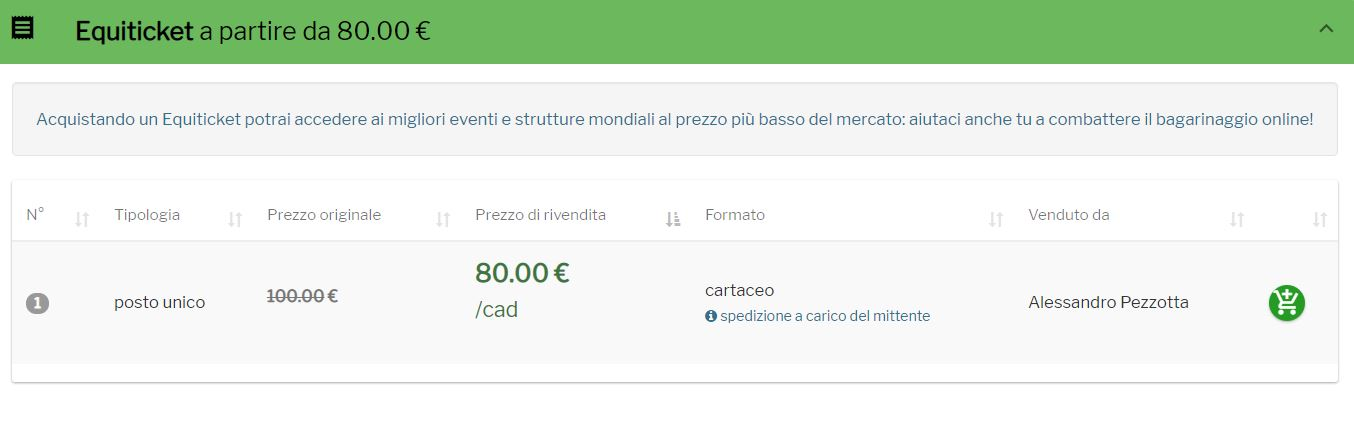
\includegraphics[width=0.68\textwidth]{chapter4/immagini/test_acquisto1}
	\caption{Inserimento nel carrello del biglietto}
	\label{testcart}
\end{figure}
\begin{figure}[htbp]
	\centering
	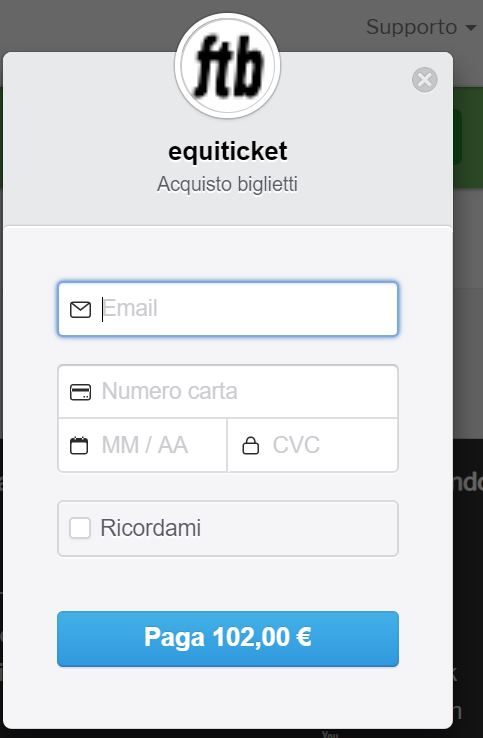
\includegraphics[width=0.68\textwidth]{chapter4/immagini/pagamento}
	\caption{Pagamento del biglietto desiderato}
	\label{testmoney}
\end{figure}
\item Una volta completato l'acquisto, viene automaticamente inviata una mail all'acquirente (Figura \ref{testmail}): 
 \begin{figure}[htbp]
	\centering
	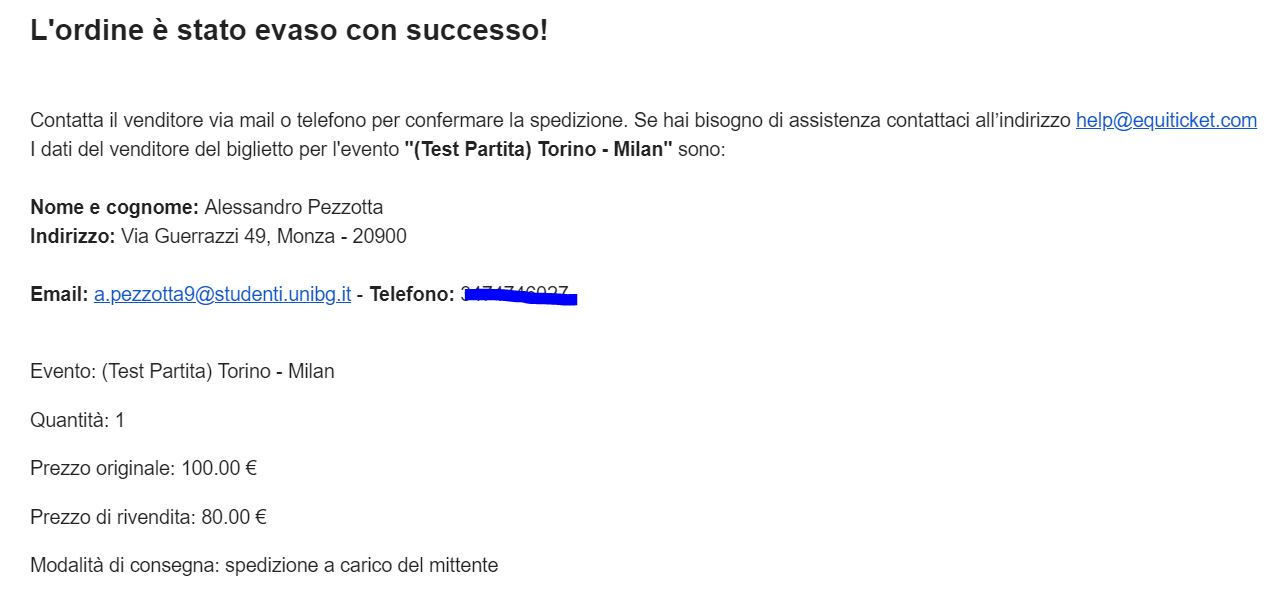
\includegraphics[width=0.68\textwidth]{chapter4/immagini/mail_acq}
	\caption{Mail automatica confermante l'avvenuto acquisto}
	\label{testmail}
\end{figure}
\end{enumerate}
\subsubsection{Dati reali di transazioni}
Data l'impossibilità di recuperare i dati di Stripe relativamente all'ambiente di test, in quanto non viene tenuta traccia delle transazioni fasulle tra Test Card, per mostrare l'effettivo funzionamento del meccanismo descritto vengono mostrate alcune transazioni relative ad eventi reali: 
\begin{enumerate}
\item \textbf{\textit{Pagamento effettuato con successo}}: i dati sono stati estrapolati da una transazione effettuata con successo per una cifra di 103,90€ (Figura \ref{stripe1} e \ref{stripe2}):  
\begin{figure}[htbp]
    \centering
    \begin{minipage}{0.45\textwidth}
        \centering
        
\includegraphics[width=0.9\textwidth]{chapter4/immagini/es_stripe} % first figure itself
        \caption{Dettaglio del pagamento}
				\label{stripe1}
    \end{minipage}\hfill
    \begin{minipage}{0.45\textwidth}
        \centering
        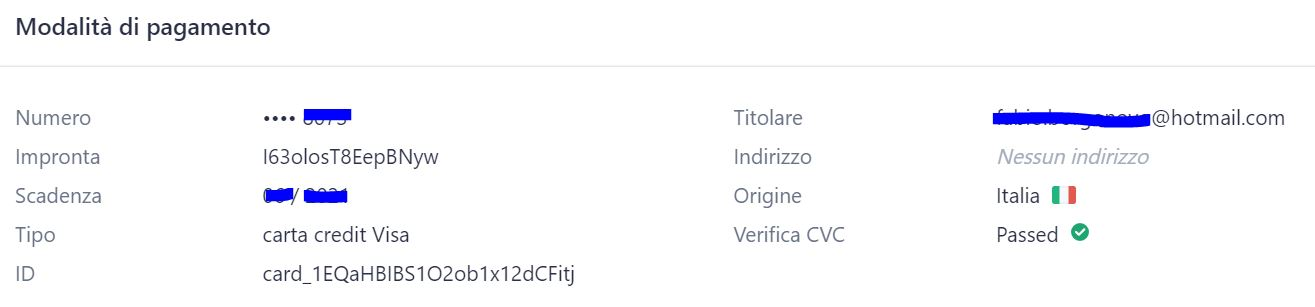
\includegraphics[width=0.9\textwidth]{chapter4/immagini/es_stripe_2} % second figure itself
        \caption{Ulteriori dettagli del pagamento}
				\label{stripe2}
    \end{minipage}
\end{figure}
\item \textbf{\textit{Cifra trattenuta ai fini di sicurezza}}: viene mostrata ora la trattenuta di una cifra di 141€ a scopo preventivo (la stessa descritta nella Sezione \ref{tratt}), che avviene nel momento in cui l'acquirente inserisce il biglietto nel carrello: la cifra viene poi rilasciata sette giorni dopo, quando il venditore avrà già provveduto alla spedizione. 
Per le trattenute, Stripe chiama la API "Authorization and Capture" senza però catturare immediatamente il pagamento: questa azione potrà essere fatta entro sette giorni, dopo i quali il Token scadrà e sarà necessario creare un altro oggetto Charge.
Si mostra il dettaglio di una trattenuta effettuata in data 18/04/2019 (screenshot effettuato il giorno stesso), in cui si mostra che il pagamento non è effettivamente stato addebitato (Figura \ref{trattreal}), ma è ancora possibile farlo (non sono ancora trascorsi sette giorni): 
\begin{figure}[htbp]
	\centering
	
\includegraphics[width=0.68\textwidth]{chapter4/immagini/es_stripe_trattenuta}
	\caption{"\emph{Test card}" utilizzata da Stripe per la creazione del Token}
	\label{trattreal}
\end{figure}
Per le transazioni avvenute in ambiente di produzione, Stripe mette a disposizione la possibilità di mostrare il corpo della API che ha generato la transazione (Figura \ref{apireal}): 
\begin{figure}[htbp]
	\centering
	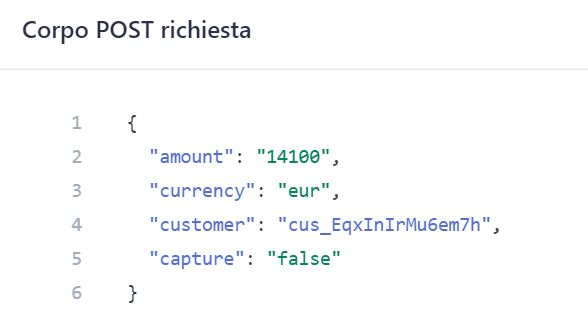
\includegraphics[width=0.68\textwidth]{chapter4/immagini/es_stripe_capture}
	\caption{Parametri con cui è stata chiamata "Authorization and Capture"}
	\label{apireal}
\end{figure}
Coerentemente con quanto dichiarato nelle sezioni precedenti, il parametro \textit{capture} impostato a \textit{false} impedisce l'addebito immediato. 
\end{enumerate}




